%  LaTeX support: latex@mdpi.com 
%  For support, please attach all files needed for compiling as well as the log file, and specify your operating system, LaTeX version, and LaTeX editor.

%=================================================================
\documentclass[cryptography,review,submit,pdftex,moreauthors,amsmath,amssymb,aps,strict]{Definitions/mdpi} 

\usepackage{mathrsfs}
\usepackage{mathtools}
\usepackage[english]{babel}
\usepackage{caption}
\usepackage{subcaption}
\usepackage{url}
\usepackage{braket}
\usepackage{algorithm}
\usepackage{algpseudocodex}
\usepackage{tikz}
\usepackage{tikz-3dplot}
\usepackage{pgfplots}
\usepackage{wasysym}
\usepackage{multirow}
\setlength{\headheight}{20.0pt}
\pgfplotsset{compat=newest}

\usetikzlibrary{positioning, fit, calc, shadows, shadows.blur, arrows.meta, shapes.geometric, fillbetween, fadings, quantikz2}

\let\oldalgorithmic\algorithmic
\let\endoldalgorithmic\endalgorithmic
\renewenvironment{algorithmic}
{\begin{adjustwidth}{-1em}{}\oldalgorithmic}
{\endoldalgorithmic\end{adjustwidth}}

\colorlet{nodeVLineColor}{blue}
\colorlet{nodeVFillColor}{cyan!20}
\colorlet{nodeULineColor}{orange}
\colorlet{nodeUFillColor}{yellow!20}
\colorlet{nodeRedLineColor}{red}
\colorlet{nodeRedFillColor}{red!20}
\colorlet{nodeGreenLineColor}{green}
\colorlet{nodeGreenFillColor}{green!20}
\colorlet{nodeBlueLineColor}{blue}
\colorlet{nodeBlueFillColor}{cyan!20}
\colorlet{nodeBlueLineColor}{blue}
\colorlet{nodeBlueFillColor}{cyan!20}
\colorlet{graphEdgeColor}{gray}
\colorlet{graphNonEdgeColor}{lightgray}
\colorlet{setDFillColor}{red!20}
\colorlet{setHFillColor}{green!20}
\colorlet{setHDFillColor}{blue!20}
\colorlet{topologyFillColor}{cyan!10}
\colorlet{blockchainDiscColor}{blue!10}
\colorlet{blockchainPendingDiscColor}{red!10}
\colorlet{redHighlightColor}{red!80}
\colorlet{blueHighlightColor}{blue!80}

\tikzset{
	genericStyle/.style = {
		every node/.style = {circle, draw, minimum size=2em}, >=latex
	}
}

\tikzset{
	myShadow/.style = {
		blur shadow = {shadow blur steps=5, shadow xshift=0.15em, shadow yshift=-0.1em}
	}
}

\tikzset{
	myLightShadow/.style = {
		blur shadow = {shadow blur steps=5, shadow xshift=0.1em, shadow yshift=-0.066em}
	}
}

\tikzset{
	nodeUStyle/.style = {
		draw=nodeULineColor, fill=nodeUFillColor, myShadow
	}
}

\tikzset{
	nodeVStyle/.style = {
		draw=nodeVLineColor, fill=nodeVFillColor, myShadow
	}
}

\tikzset{
	nodeGrayStyleC/.style = {
		draw=gray, fill=gray!20, myShadow
	}
}

\tikzset{
	nodeGrayStyle/.style = {
		draw=black, fill=gray!20, myShadow
	}
}

\tikzset{
	nodeLightGrayStyle/.style = {
		draw=gray, fill=lightgray!20, myShadow
	}
}

\tikzset{
	nodeRedStyle/.style = {
		draw=nodeRedLineColor, line width=0.25, line cap=round, fill=nodeRedFillColor, myLightShadow
	}
}

\tikzset{
	nodeBlueStyle/.style = {
		draw=nodeBlueLineColor, line width=0.25, line cap=round, fill=nodeBlueFillColor
	}
}

\tikzset{
	graphEdgeStyle/.style = {
		draw=graphEdgeColor, line width=1, line cap=round
	}
}
	
\tikzset{
	graphNonEdgeStyle/.style = {
		draw=graphNonEdgeColor, opacity=0.25, line width=1, line cap=round
	}
}

\tikzset{
	graphRedEdgeStyle/.style = {
		draw=red, opacity=0.5, line width=1.5, line cap=round
	}
}

\tikzset{
	graphLightRedEdgeStyle/.style = {
		draw=nodeRedLineColor, opacity=0.15
	}
}

\tikzset{
	graphBlueEdgeStyle/.style = {draw=blue!50, line width=0.5}
}

\frenchspacing

\captionsetup[figure]{margin=0pt, font=small, labelfont=bf, labelsep=endash, justification=centerlast, labelsep=colon}
\captionsetup[algorithm]{margin=0pt, font=small, labelfont=bf, labelsep=endash, justification=centerlast, labelsep=colon}
\usepackage{pifont}% http://ctan.org/pkg/pifont
\newcommand{\cmark}{\ding{51}}%
\newcommand{\xmark}{\ding{55}}%

\newcommand{\peter}[1]{\textcolor{red}{#1}}
\newcommand{\minh}[1]{\textcolor{blue}{#1}}


%--------------------
% Class Options:
%--------------------
%----------
% journal
%----------
% Choose between the following MDPI journals:
% acoustics, actuators, addictions, admsci, adolescents, aerobiology, aerospace, agriculture, agriengineering, agrochemicals, agronomy, ai, air, algorithms, allergies, alloys, analytica, analytics, anatomia, animals, antibiotics, antibodies, antioxidants, applbiosci, appliedchem, appliedmath, applmech, applmicrobiol, applnano, applsci, aquacj, architecture, arm, arthropoda, arts, asc, asi, astronomy, atmosphere, atoms, audiolres, automation, axioms, bacteria, batteries, bdcc, behavsci, beverages, biochem, bioengineering, biologics, biology, biomass, biomechanics, biomed, biomedicines, biomedinformatics, biomimetics, biomolecules, biophysica, biosensors, biotech, birds, bloods, blsf, brainsci, breath, buildings, businesses, cancers, carbon, cardiogenetics, catalysts, cells, ceramics, challenges, chemengineering, chemistry, chemosensors, chemproc, children, chips, cimb, civileng, cleantechnol, climate, clinpract, clockssleep, cmd, coasts, coatings, colloids, colorants, commodities, compounds, computation, computers, condensedmatter, conservation, constrmater, cosmetics, covid, crops, cryptography, crystals, csmf, ctn, curroncol, cyber, dairy, data, ddc, dentistry, dermato, dermatopathology, designs, devices, diabetology, diagnostics, dietetics, digital, disabilities, diseases, diversity, dna, drones, dynamics, earth, ebj, ecologies, econometrics, economies, education, ejihpe, electricity, electrochem, electronicmat, electronics, encyclopedia, endocrines, energies, eng, engproc, entomology, entropy, environments, environsciproc, epidemiologia, epigenomes, est, fermentation, fibers, fintech, fire, fishes, fluids, foods, forecasting, forensicsci, forests, foundations, fractalfract, fuels, future, futureinternet, futurepharmacol, futurephys, futuretransp, galaxies, games, gases, gastroent, gastrointestdisord, gels, genealogy, genes, geographies, geohazards, geomatics, geosciences, geotechnics, geriatrics, grasses, gucdd, hazardousmatters, healthcare, hearts, hemato, hematolrep, heritage, higheredu, highthroughput, histories, horticulturae, hospitals, humanities, humans, hydrobiology, hydrogen, hydrology, hygiene, idr, ijerph, ijfs, ijgi, ijms, ijns, ijpb, ijtm, ijtpp, ime, immuno, informatics, information, infrastructures, inorganics, insects, instruments, inventions, iot, j, jal, jcdd, jcm, jcp, jcs, jcto, jdb, jeta, jfb, jfmk, jimaging, jintelligence, jlpea, jmmp, jmp, jmse, jne, jnt, jof, joitmc, jor, journalmedia, jox, jpm, jrfm, jsan, jtaer, jvd, jzbg, kidneydial, kinasesphosphatases, knowledge, land, languages, laws, life, liquids, literature, livers, logics, logistics, lubricants, lymphatics, machines, macromol, magnetism, magnetochemistry, make, marinedrugs, materials, materproc, mathematics, mca, measurements, medicina, medicines, medsci, membranes, merits, metabolites, metals, meteorology, methane, metrology, micro, microarrays, microbiolres, micromachines, microorganisms, microplastics, minerals, mining, modelling, molbank, molecules, mps, msf, mti, muscles, nanoenergyadv, nanomanufacturing,\gdef\@continuouspages{yes}} nanomaterials, ncrna, ndt, network, neuroglia, neurolint, neurosci, nitrogen, notspecified, %%nri, nursrep, nutraceuticals, nutrients, obesities, oceans, ohbm, onco, %oncopathology, optics, oral, organics, organoids, osteology, oxygen, parasites, parasitologia, particles, pathogens, pathophysiology, pediatrrep, pharmaceuticals, pharmaceutics, pharmacoepidemiology,\gdef\@ISSN{2813-0618}\gdef\@continuous pharmacy, philosophies, photochem, photonics, phycology, physchem, physics, physiologia, plants, plasma, platforms, pollutants, polymers, polysaccharides, poultry, powders, preprints, proceedings, processes, prosthesis, proteomes, psf, psych, psychiatryint, psychoactives, publications, quantumrep, quaternary, qubs, radiation, reactions, receptors, recycling, regeneration, religions, remotesensing, reports, reprodmed, resources, rheumato, risks, robotics, ruminants, safety, sci, scipharm, sclerosis, seeds, sensors, separations, sexes, signals, sinusitis, skins, smartcities, sna, societies, socsci, software, soilsystems, solar, solids, spectroscj, sports, standards, stats, std, stresses, surfaces, surgeries, suschem, sustainability, symmetry, synbio, systems, targets, taxonomy, technologies, telecom, test, textiles, thalassrep, thermo, tomography, tourismhosp, toxics, toxins, transplantology, transportation, traumacare, traumas, tropicalmed, universe, urbansci, uro, vaccines, vehicles, venereology, vetsci, vibration, virtualworlds, viruses, vision, waste, water, wem, wevj, wind, women, world, youth, zoonoticdis 
% For posting an early version of this manuscript as a preprint, you may use "preprints" as the journal. Changing "submit" to "accept" before posting will remove line numbers.

%---------
% article
%---------
% The default type of manuscript is "article", but can be replaced by: 
% abstract, addendum, article, book, bookreview, briefreport, casereport, comment, commentary, communication, conferenceproceedings, correction, conferencereport, entry, expressionofconcern, extendedabstract, datadescriptor, editorial, essay, erratum, hypothesis, interestingimage, obituary, opinion, projectreport, reply, retraction, review, perspective, protocol, shortnote, studyprotocol, systematicreview, supfile, technicalnote, viewpoint, guidelines, registeredreport, tutorial
% supfile = supplementary materials

%----------
% submit
%----------
% The class option "submit" will be changed to "accept" by the Editorial Office when the paper is accepted. This will only make changes to the front page (e.g., the logo of the journal will get visible), the headings, and the copyright information. Also, line numbering will be removed. Journal info and pagination for accepted papers will also be assigned by the Editorial Office.

%------------------
% moreauthors
%------------------
% If there is only one author the class option oneauthor should be used. Otherwise use the class option moreauthors.

%---------
% pdftex
%---------
% The option pdftex is for use with pdfLaTeX. Remove "pdftex" for (1) compiling with LaTeX & dvi2pdf (if eps figures are used) or for (2) compiling with XeLaTeX.

%=================================================================
% MDPI internal commands - do not modify
\firstpage{1} 
\makeatletter 
\setcounter{page}{\@firstpage} 
\makeatother
\pubvolume{1}
\issuenum{1}
\articlenumber{0}
\pubyear{2024}
\copyrightyear{2024}
%\externaleditor{Academic Editor: Firstname Lastname}
\datereceived{ } 
\daterevised{ } % Comment out if no revised date
\dateaccepted{ } 
\datepublished{ } 
%\datecorrected{} % For corrected papers: "Corrected: XXX" date in the original paper.
%\dateretracted{} % For corrected papers: "Retracted: XXX" date in the original paper.
\hreflink{https://doi.org/} % If needed use \linebreak
%\doinum{}
%\pdfoutput=1 % Uncommented for upload to arXiv.org
%\CorrStatement{yes}  % For updates


%=================================================================
% Add packages and commands here. The following packages are loaded in our class file: fontenc, inputenc, calc, indentfirst, fancyhdr, graphicx, epstopdf, lastpage, ifthen, float, amsmath, amssymb, lineno, setspace, enumitem, mathpazo, booktabs, titlesec, etoolbox, tabto, xcolor, colortbl, soul, multirow, microtype, tikz, totcount, changepage, attrib, upgreek, array, tabularx, pbox, ragged2e, tocloft, marginnote, marginfix, enotez, amsthm, natbib, hyperref, cleveref, scrextend, url, geometry, newfloat, caption, draftwatermark, seqsplit
% cleveref: load \crefname definitions after \begin{document}

%=================================================================
% Please use the following mathematics environments: Theorem, Lemma, Corollary, Proposition, Characterization, Property, Problem, Example, ExamplesandDefinitions, Hypothesis, Remark, Definition, Notation, Assumption
%% For proofs, please use the proof environment (the amsthm package is loaded by the MDPI class).

%=================================================================
% Full title of the paper (Capitalized)
\Title{REVIEW ON IPQ-LWE-TCFs}

% MDPI internal command: Title for citation in the left column
\TitleCitation{Title}

% Author Orchid ID: enter ID or remove command
\newcommand{\orcidauthorA}{0000-0000-0000-000X} % Add \orcidA{} behind the author's name
%\newcommand{\orcidauthorB}{0000-0000-0000-000X} % Add \orcidB{} behind the author's name

% Authors, for the paper (add full first names)
\Author{Firstname Lastname $^{1,\dagger,\ddagger}$\orcidA{}, Firstname Lastname $^{2,\ddagger}$ and Firstname Lastname $^{2,}$*}

%\longauthorlist{yes}

% MDPI internal command: Authors, for metadata in PDF
\AuthorNames{Firstname Lastname, Firstname Lastname and Firstname Lastname}

% MDPI internal command: Authors, for citation in the left column
\AuthorCitation{Lastname, F.; Lastname, F.; Lastname, F.}
% If this is a Chicago style journal: Lastname, Firstname, Firstname Lastname, and Firstname Lastname.

% Affiliations / Addresses (Add [1] after \address if there is only one affiliation.)
\address{%
$^{1}$ \quad Affiliation 1; e-mail@e-mail.com\\
$^{2}$ \quad Affiliation 2; e-mail@e-mail.com}

% Contact information of the corresponding author
\corres{Correspondence: e-mail@e-mail.com; Tel.: (optional; include country code; if there are multiple corresponding authors, add author initials) +xx-xxxx-xxx-xxxx (F.L.)}

% Current address and/or shared authorship
\firstnote{Current address: Affiliation.}  % Current address should not be the same as any items in the Affiliation section.
\secondnote{These authors contributed equally to this work.}
% The commands \thirdnote{} till \eighthnote{} are available for further notes

%\simplesumm{} % Simple summary

%\conference{} % An extended version of a conference paper

% Abstract (Do not insert blank lines, i.e. \\) 
\abstract{The recent development of quantum computers poses a significant threat to classical cryptographic systems, necessitating a collaborative effort between quantum computing and cryptography researchers. This review aims to bridge the gap between these fields by providing an accessible overview of Proof of Quantumness (PQ), Trapdoor Claw-free Functions, and the Learning with Errors (LWE) problem for those not experienced in both areas. The PQ protocol offers a method for a classical verifier to validate the quantum capabilities of a quantum prover. Additionally, we explore the definition and applications of Trapdoor Claw-free Functions in constructing quantum-resistant cryptographic protocols and give a brief overview of the foundational aspects of the LWE problem in post-quantum cryptography. Our review underscores the necessity for knowledge exchange between QC and cryptography communities in the quantum era by presenting these complex topics in an approachable manner.
}

% Keywords
\keyword{interactive proof of quantumness, trapdoor claw-free function, lattice, lwe} 

% The fields PACS, MSC, and JEL may be left empty or commented out if not applicable
%\PACS{J0101}
%\MSC{}
%\JEL{}

%%%%%%%%%%%%%%%%%%%%%%%%%%%%%%%%%%%%%%%%%%
% Only for the journal Diversity
%\LSID{\url{http://}}

%%%%%%%%%%%%%%%%%%%%%%%%%%%%%%%%%%%%%%%%%%
% Only for the journal Applied Sciences
%\featuredapplication{Authors are encouraged to provide a concise description of the specific application or a potential application of the work. This section is not mandatory.}
%%%%%%%%%%%%%%%%%%%%%%%%%%%%%%%%%%%%%%%%%%

%%%%%%%%%%%%%%%%%%%%%%%%%%%%%%%%%%%%%%%%%%
% Only for the journal Data
%\dataset{DOI number or link to the deposited data set if the data set is published separately. If the data set shall be published as a supplement to this paper, this field will be filled by the journal editors. In this case, please submit the data set as a supplement.}
%\datasetlicense{License under which the data set is made available (CC0, CC-BY, CC-BY-SA, CC-BY-NC, etc.)}

%%%%%%%%%%%%%%%%%%%%%%%%%%%%%%%%%%%%%%%%%%
% Only for the journal Toxins
%\keycontribution{The breakthroughs or highlights of the manuscript. Authors can write one or two sentences to describe the most important part of the paper.}

%%%%%%%%%%%%%%%%%%%%%%%%%%%%%%%%%%%%%%%%%%
% Only for the journal Encyclopedia
%\encyclopediadef{For entry manuscripts only: please provide a brief overview of the entry title instead of an abstract.}

%%%%%%%%%%%%%%%%%%%%%%%%%%%%%%%%%%%%%%%%%%
% Only for the journal Advances in Respiratory Medicine
%\addhighlights{yes}
%\renewcommand{\addhighlights}{%

%\noindent This is an obligatory section in “Advances in Respiratory Medicine”, whose goal is to increase the discoverability and readability of the article via search engines and other scholars. Highlights should not be a copy of the abstract, but a simple text allowing the reader to quickly and simplified find out what the article is about and what can be cited from it. Each of these parts should be devoted up to 2~bullet points.\vspace{3pt}\\
%\textbf{What are the main findings?}
% \begin{itemize}[labelsep=2.5mm,topsep=-3pt]
% \item First bullet.
% \item Second bullet.
% \end{itemize}\vspace{3pt}
%\textbf{What is the implication of the main finding?}
% \begin{itemize}[labelsep=2.5mm,topsep=-3pt]
% \item First bullet.
% \item Second bullet.
% \end{itemize}
%}

%%%%%%%%%%%%%%%%%%%%%%%%%%%%%%%%%%%%%%%%%%
\begin{document}

%%%%%%%%%%%%%%%%%%%%%%%%%%%%%%%%%%%%%%%%%%
\section{Introduction} \label{introduction}

\subsection{Overview of Quantum Computing and Post-quantum Cryptography}

Quantum computing represents a transformative leap in computational capabilities, using the principles of quantum mechanics to process information in fundamentally new ways. Unlike classical computers, which use bits as the smallest unit of data, quantum computers use quantum bits or qubits. These qubits do not exist in a specific state but in a superposition of multiple states, enabling quantum computers to perform certain computations exponentially faster than their classical counterparts. 

The need for secure communication has been a constant throughout history, driving the development of cryptographic techniques to protect sensitive information. The security of classical cryptography largely relies on mathematical problems assumed to be computationally hard to solve. These problems, such as integer factorization and the discrete logarithm problem, form the basis of widely used algorithms like RSA and ECC. However, the development of quantum computing presents a significant challenge. Shor's algorithm \cite{Shor94}, for example, can efficiently solve the problems mentioned above, making these cryptographic primitives vulnerable to future quantum attacks. While not all classical cryptographic primitives are vulnerable to these attacks, RSA/ECC form the basis of contemporary public-key infrastructure, essential to the functionality of the internet.

In recent years, the rapid development of quantum computing has raised major security concerns in these cryptographic schemes. Consequently, post-quantum cryptography (PQC) is now a thriving field with the view of developing new cryptographic constructions secure against classical and quantum attacks, often referred to as `quantum resistance'. In the context of post-quantum cryptography, many approaches are using different building blocks: \textit{hash-based, code-based, multivariate-based, isogeny-based and lattice-based schemes:}
\begin{itemize}
    \item Hash-based cryptography: Utilising the hard-to-invert property of hash functions to build digital signature schemes.
    \item Code-based constructions derive their security from decoding generic linear codes.
    \item Multivariate-based cryptography uses the NP-hard Multivariate Quadratic Problem (MQ Problem) over finite fields $\mathbb{F}_p$ to construct cryptosystems.
    \item Isogeny-based cryptography is the youngest field whose constructions are based on the hardness of finding special maps called isogenies between supersingular elliptic curves.
    \item Lattice-based cryptography is based on the computational difficulty of mathematical problems associated with lattices: short integer solution (SIS), learning with errors (LWE), and their variants.
\end{itemize}

Lattice-based cryptography is arguably the most promising branch in post-quantum cryptography today due to its versatility, supporting a wide range of symmetric and asymmetric cryptographic primitives including digital signatures and public-key encryption. Additionally, lattice-based techniques are computationally efficient with compact key sizes.

Another significant field that has emerged in recent years is quantum cryptography, which has a major impact on symmetric key encryption constructions by achieving information-theoretic security. An example of this is Quantum Key Distribution (QKD)~\cite{BB84,E91}, a technique that allows two parties to generate a shared secret key, which can then be used for symmetric encryption. QKD leverages the principles of quantum mechanics to ensure that any attempt at eavesdropping on the key exchange can be detected; hence providing a level of security called information-theoretic security.
%that is theoretically unbreakable by any computational means.

However, this does not apply to asymmetric key encryption because one of the keys always remains public. For asymmetric constructions, developing post-quantum cryptography (PQC) is still the main research goal. Based on "hard-to-solve" assumptions, PQC faces the same problem as classical cryptography, i.e., computational security.

\subsection{Communication between a quantum computer and classical devices.}

The focus of this review is on the proof of quantumness, which explores the intersection between the classical and quantum realms, where communication between a quantum computer and classical devices is a critical aspect of integrating quantum technology into existing frameworks. This interaction often requires protocols that allow classical devices to verify the quantum power of other devices. One such protocol is the Proof of Quantumness (PQ), which provides a method for a classical verifier to interact with a quantum prover. The PQ protocol ensures that the quantum device can demonstrate its quantum capabilities by performing computations that are infeasible for classical devices, thereby establishing a proof of quantumness. This verification is essential for tasks where quantum advantages need to be reliably authenticated, such as in secure communications and advanced cryptographic protocols. By bridging the gap between quantum and classical worlds, PQ protocol facilitates the trust and usability of quantum computers in practical applications.

One recent approach is to use Trapdoor Claw-free functions to build Proof of Quantumness protocols. Note that Trapdoor Claw-free functions still base their security on hard problems like learning with errors (LWE) and ring learning with errors (RLWE), making them computationally secure but not information-theoretically secure.

\subsection{Notation}

The following notations are used throughout this paper:
\begin{itemize}
    \item $q$: prime integer;
    \item $\lambda$: security parameter;
    \item $\mathbb{N}$: the set of natural numbers;
    \item $\mathbb{Z}$: the set of integers;
    \item $\mathbb{Z}_p$: the ring of integers modulo $p$;
    \item $x\gets S$: the action of sampling a uniformly random element $x$ from the set $S$;
    \item $p(n)$ a polynomial function associated with the security parameter $n$. A function $\mathrm{negl}(n)$ is said to be negligible if $\mathrm{negl}(n)$ is smaller than all polynomial fractions for sufficiently large $n$. We define an event to occur with overwhelming probability when its probability of occurrence is at least $1-\mathrm{negl}(n)$. 
    %\peter{If $p(\lambda)$ is a polynomial then it isn't a negligible function? Should we here separately define the notion of a negligible function $\mathrm{neg}(\lambda)$?}
    \item Vectors are represented using lowercase bold letters (e.g. $\mathbf{s}$), while matrices are represented in uppercase bold (e.g. $\mathbf{A}$). 
    \item The inner product of vectors is denoted using angular brackets, e.g. $\langle\mathbf{a},\mathbf{s}\rangle$.
    \item The transpose of a vector or matrix is denoted using a superscript `T', e.g. $\mathbf{s}^T$ or $\mathbf{A}^T$, respectively.
    \item $\|\cdot\|$ denotes the Euclidean norm, $\|\cdot\|_{\infty}$ denotes the infinity norm (the absolute value of the largest component of the vector)
    %\item \textcolor{red}{Dirac notation}
    \item $\mathcal{L}(\mathbf{A})$: a lattice with basis $\mathbf{A}$.
    \item For a function $f:X\to \mathbb{R}$ over a finite domain $X$, the support of $f$, denoted by $\mathsf{SUPP}$, is the set of points in $X$ where $f$ is non-zero,
    $$\mathsf{SUPP}(f)=\{x\in X|f(x)\neq 0\}.$$
\end{itemize}
%%%%%%%%%%%%%%%%%%%%%%%%%%%%%%%%%%%%%%%%%%
\section{Quantum computing and communications} \label{quantum_computing}
\subsection{Quantum states}

In quantum mechanics, a \textit{quantum state} is a unit vector in the complex space $\mathbb{C}^N$.
As in classical computing, all computations are performed using classical bits, $0$ and $1$. In quantum computing, we use an equivalent term that has more interesting properties: the \textit{quantum bit} or \textit{qubit}. A qubit, a two-level system, can be considered the simplest unit of quantum information. Let us use Dirac notation and denote $\ket{0}$ and $\ket{1}$ as the two basis states of a qubit, similar to the classical case. The $\ket{0}$ and $\ket{1}$ are called `kets', more explanation about the use of this notation will be proposed soon in this section.

The first special property of a quantum state is \textit{superposition}, where a quantum system is not necessarily in one specific state but can be in a \textit{superposition} of them. Hence, a quantum state $\ket{\psi}$ can be expressed as a linear combination of the two basis states $\ket{0}$ and $\ket{1}$,
\begin{align}
\ket{\psi}=\alpha\ket{0}+\beta\ket{1}
\label{eq:quantumstate}
\end{align}
where the coefficients $\alpha$ and $\beta$ are complex numbers called amplitudes, and the pair $\{\ket{0},\ket{1}\}$ is orthogonal and is called computational basis.


\noindent Recall that quantum states can be written as vectors in complex space; hence, using the Dirac notation for describing quantum states simplifies linear algebra operations while working with these states. Note that kets are column vectors, for example:
\begin{align}
    \ket{0}=\begin{bmatrix} 1\\ 0
\end{bmatrix} \text{, }\ket{1}=\begin{bmatrix} 0\\1
\end{bmatrix}
\end{align}
The superposition state~\eqref{eq:quantumstate} can be represented as the following vector:
\begin{align}
    \ket{\psi}=\alpha\ket{0}+\beta\ket{1} = \begin{bmatrix} \alpha\\ \beta
\end{bmatrix}.
\end{align}

Working with row vectors in complex vector space, we also need to deal with \textit{conjugate transpose}, ie. row vectors. In the Dirac notation, these row vectors are called ``bras'', for example
\begin{align}
    \bra{0}= \begin{bmatrix} 1 & 0 \end{bmatrix} \text{, }\bra{1}=\begin{bmatrix} 0 & 1
\end{bmatrix},
\end{align}
and 
\begin{align}
    \bra{\psi}=  \begin{bmatrix} \alpha^* & \beta^*\end{bmatrix}
\end{align}
where $\alpha^*$ and $\beta^*$ are complex conjugates of $\alpha$ and $\beta$.

Another property of quantum states is \textit{measurement} where it helps one ascertain information about the quantum states. When one measures the state $\ket{\psi}$ in the computational basis, the state will \textit{collapse} to one of its possible outcomes, either $\ket{0}$ or $\ket{1}$, effectively converting quantum information into classical information. The amplitudes $\alpha$ and $\beta$ now represent the probability of obtaining the corresponding results, where $|\alpha|^2$ is the probability of collapsing to $\ket{0}$ and $|\beta|^2$  is the probability of collapsing to $\ket{0}$. For this reason, we have that the measurement result is probabilistic and not predetermined.

\begin{align}
\Pr[0] &= |\alpha|^2,\nonumber\\
\Pr[1] &= |\beta|^2,\nonumber\\
|\alpha|^2 + |\beta|^2 &= 1.
\label{eq:probability_quantum_state}
\end{align}
This collapse of quantum states is not reversible, meaning once the measurement is made, the original superposition state is lost, and we are left with classical information. This property of quantum measurement underlies many quantum algorithms and cryptographic protocols, impacting how information is extracted from quantum systems and ensuring that certain quantum properties, like entanglement and superposition, can be harnessed effectively only until the measurement is performed.

\begin{figure}[!htbp]
    \center
    \begin{quantikz}
    \lstick{$\ket{\psi}$\\initial state} & \qw
    & \meter{0/1} & \rstick{$m$} \setwiretype{c}
    \end{quantikz}
    \caption{Measuring a quantum state:  The thin line denotes quantum information and the double lines denote classical information. The result of the measurement $m$ is a classical result according to a probability distribution~\eqref{eq:probability_quantum_state}.}
    \label{fig:measurement}
\end{figure}


In quantum computing, basis quantum gates are fundamental operations used to manipulate qubits, similar to classical logic gates in classical computing. These quantum gates are represented by unitary matrices $\mathbf{U}$, which preserve the norm of quantum states and ensure reversibility. A matrix $\mathbf{U}$ is called unitary if and only if it satisfies
\begin{align}
    \mathbf{U}\mathbf{U}^{\dagger}=\mathbf{U}^{\dagger}\mathbf{U}=\mathbf{I},
\end{align}
where $\mathbf{U}^{\dagger}$ is the conjugate transpose of $\mathbf{U}$.
Among the most important of these quantum gates are the Pauli gates and the Hadamard gate. The Pauli gates consist of the Pauli-X, Pauli-Y, and Pauli-Z gates. The Pauli-X gate, represented by the matrix 
\begin{align}
    X=\begin{bmatrix} 
    0 & 1\\
    1 & 0
\end{bmatrix}
\end{align}
which functions as a quantum equivalent of the classical NOT gate, flipping the state of a qubit from $\ket{0}$ to $\ket{1}$ and vice versa. Concretely,
\begin{align}
X\ket{\psi}=X(\alpha\ket{0}+\beta\ket{1})=\alpha\ket{1}+\beta\ket{0}.
\end{align}
\noindent The Pauli-Z gate, represented by the matrix
\begin{align}
    Z=\begin{bmatrix} 
    1 & 0\\
    0 & -1
\end{bmatrix}
\end{align}
performs a phase-flip, changing the sign of the $\ket{1}$ state while leaving the $\ket{0}$ state unchanged:
\begin{align}
Z\ket{\psi}=Z(\alpha\ket{0}+\beta\ket{1})=\alpha\ket{0}-\beta\ket{1}.
\end{align}
The Pauli-Y gate, represented by the matrix 
\begin{align}
    Y=\begin{bmatrix} 
    0 & -i\\
    i & 0
\end{bmatrix}
\end{align}
combines a bit-flip and a phase-flip.

\noindent The Hadamard gate $H$, another essential quantum gate, is represented by the matrix 
\begin{align}
    H=\frac{1}{\sqrt{2}}\begin{bmatrix} 
    1 & 1\\
    1 & 0
\end{bmatrix}.
\end{align}
This gate transforms the computational basis states into equal superpositions of $\ket{0}$ and $\ket{1}$, where
\begin{align}
    H\ket{0}=\frac{\ket{0}+\ket{1}}{\sqrt{2}}=\ket{+},\\
    H\ket{1}=\frac{\ket{0}-\ket{1}}{\sqrt{2}}=\ket{-}.
\end{align}

When discussing measurements in quantum computing, we consider a specific property of the qubit, and using different bases yields varied outcomes, similar to how measuring classical objects differs based on what is being measured. While the computational basis $(\ket{0},\ket{1})$ is commonly used, other bases, like the Hadamard basis $\{\ket{+},\ket{-}\}$, are also important. For example, measuring the state $\ket{\psi}=\alpha\ket{0}+\beta\ket{1}$ using the Hadamard basis, the state will collapse to either $\ket{+}$ or $\ket{-}$ with probability $|\alpha+\beta|^2/2$ and $|\alpha-\beta|^2/2$, respectively. 

\subsection{Hadamard Transform and Quantum Parallelism}
Note that when one applies the Hadamard gate to each qubit in an $n$-qubit system, each initialized to $\ket{0}$, it creates a uniform superposition of all possible  $2^n$ superposition, represented as  
\begin{align}
    H^{\otimes n}\ket{\mathbf{0}}=\frac{1}{\sqrt{2}^n}\sum_{\mathbf{x}\in\{0,1\}^n}\ket{\mathbf{x}}.
\end{align}

\begin{figure}[!htbp]
    \center
    \begin{quantikz}
\lstick{$\ket{\mathbf{0}}$} &[4em] \gate{H^{\otimes n}}\qwbundle
{n} & \qw
\end{quantikz}
    \caption{Quantum circuit applying the Hadamard transform to $n$-qubit system.}
    \label{fig:fig:hadamard-transform}
\end{figure}

This superposition is crucial for quantum computing because it allows a quantum computer to process multiple inputs simultaneously. Note that in quantum computing, a register is a collection of qubits where different registers within a quantum system can serve various purposes. For example, the input registers hold the initial state of the input data for a quantum computation while the output register is where the results of the quantum computation are stored. After the quantum algorithm has been executed, measuring the qubits in the output register collapses their state to classical bits, providing the final result of the computation.

When a function $f(\mathbf{x})$ is evaluated on the aforementioned input register, it effectively evaluates the function for all possible inputs $\mathbf{x}$ in parallel, which significantly enhances the computational power of quantum computers. This phenomenon is also called quantum parallelism. Concretely, one first uses an auxiliary qubit register (initialized to $\ket{0}$) to store the function's output then uses a quantum circuit evaluating the classical function $U_f$ that maps each basis state $\ket{\mathbf{x}}$ to $\ket{\mathbf{x}}\ket{f(\mathbf{x})}$:
\begin{align}
U_f\Bigl(\frac{1}{\sqrt{2}^n}\sum_{\mathbf{x}\in\{0,1\}^n}\ket{\mathbf{x}}\ket{0}\Bigr) = \frac{1}{\sqrt{2}^n}\sum_{\mathbf{x}\in\{0,1\}^n}\ket{\mathbf{x}}\ket{f(\mathbf{x})}
\end{align}

By measuring the output register, which holds $f(\mathbf{x})$, one can obtain the function's value for a specific input $\mathbf{x}$. 
\begin{figure}[!htbp]
    \center
    \begin{quantikz}
        \setwiretype{n} & & \lstick{$\ket{\mathbf{0}}$} & \setwiretype{q} \qwbundle{n} & \gate{H^{\otimes n}} & \gate[2][5em]{U_f}\gateinput{$\mathbf{x}$}\gateoutput{$\mathbf{x}$} & & &  \\
\setwiretype{n} & & \lstick{$\ket{\mathbf{0}}$} & \setwiretype{q} \qwbundle{n-1} & & \gateinput{$\mathbf{y}$}\gateoutput{$\mathbf{y}\oplus f(\mathbf{x})$} & \qwbundle{n-1} & \meter{} & \setwiretype{c} \rstick{$\mathbf{w}$} & \setwiretype{n}
    \end{quantikz}
    \caption{Evaluation of a classical function $f(\mathbf{x})$ on quantum registers.}
    \label{fig:quantum_parallelism}
\end{figure}


%This ``weird'' property of qubits makes the idea of quantum computers more promising since with $n$ classical bits, one can perform up to $n$ computations, while with $n$ qubits, this number could reach up to $2^n$ superposition. \peter{Not computations, rather terms in the superposition}.

\subsection{No-cloning theorem}

The no-cloning theorem is a fundamental principle in quantum mechanics that states it is impossible to create an exact copy of an arbitrary unknown quantum state. The no-cloning theorem has a profound impact on cryptography, especially in quantum key distribution (QKD). The security of the BB84 protocol~\cite{BB84}, a well-known QKD construction, relies on the impossibility of an adversary perfectly cloning the quantum states, preventing them from interfering with the states being transferred between honest parties. Furthermore, any attempt to clone a quantum state by measuring it would collapse the state, exposing the eavesdropper's existence.

%%%%%%%%%%%%%%%%%%%%%%%%%%%%%%%%%%%%%%%%%%

\section{Lattice-based post-quantum cryptography} \label{post-quantum-cryptography-pqc}

\subsection{Lattices}
\subsubsection{Definitions}\label{lattice}
\begin{Definition}
    Lattices in $\mathbb{R}^n$ are sets of linear combinations for some basis. Concretely, consider integer lattice $\mathcal{L}\subseteq \mathbb{Z}^n$, $\mathcal{L}$ can be represented by a basis $\mathbf{A}=[\mathbf{a}_1,\cdots,\mathbf{a}_n]\in\mathbb{Z}^{m\times n}$, where each vector $\mathbf{a}_i$ is written in column form as follow: 

\begin{align}
    \mathcal{L}(\mathbf{A}):=\left\{\sum_{i=1}^n\mathbf{a}_i x_i | x_i\in\mathbb{Z}~\forall i=1,\cdots,n \right\}\subseteq\mathbb{Z}^m.
\end{align}
\end{Definition}

We refer to $n$ as the rank of the lattice $\mathcal{L}$ and $m$ as its dimension. $\mathcal{L}$ is called a full-rank lattice if $n=m$. In most lattice-based cryptographic constructions, we primarily utilize full-rank lattices that include $q\mathbb{Z}^m$, known as $q$-ary lattices lattices, which are defined as follows 
\begin{align}
%\mathcal{L}_q(\mathbf{A}) &:= \left\{ \mathbf{x}\in\mathbb{Z}^m ~\rm{s.t.}~ \mathbf{x}\mod q \in\mathbf{A}^T\mathbb{Z}^n_q \right\}\\
\mathcal{L}_q(\mathbf{A}) &:= \left\{ \mathbf{x}\in\mathbb{Z}^m ~\rm{s.t.}~\exists \mathbf{s}\in\mathbb{Z}_q^n~\rm{where}~\mathbf{A}^T\mathbf{s}=\mathbf{x}\mod q \right\}\\
\mathcal{L}^{\perp}_q(\mathbf{A}) &:= \left\{  \mathbf{x}\in\mathbb{Z}^m~\rm{s.t.}~\mathbf{A}\mathbf{x}=0\mod q \right\} 
\end{align}

However, to simplify the notation, we will omit $q$ and simply write $\mathcal{L}(\mathbf{A})$ and $\mathcal{L}^{\perp}(\mathbf{A})$ for a given matrix $\mathbf{A}$. 


Consider a basis $\mathbf{A}$ of $\mathcal{L}$, we called $P(\mathbf{A})=\{\mathbf{A}\mathbf{x}|\mathbf{x}\in[0,1)^n\}$ is the fundamental parallelepiped of $\mathbf{A}$. A ``good'' basis of $\mathcal{L}$ results in a parallelepiped that is more square-like, whereas a ``bad'' basis produces a very thin parallelepiped. We denote$\|\mathbf{A}\|:=\max_{1 \le i \le k} \|\mathbf{a}_i\|$ the maximum $l_2$ length of the vectors in $\mathbf{A}$ and $\tilde{\mathbf{A}}:=\{\tilde{\mathbf{a}}_1,\cdots,\tilde{\mathbf{a}}_k \}$ the Gram-Schmidt orthogonalization of the vectors $\mathbf{a}_1,\cdots,\mathbf{a}_k$ in that order.


\begin{figure}[!htb]
    \centering
    \begin{tikzpicture}
    \coordinate (Origin)   at (0,0);
    \coordinate (XAxisMin) at (-3,0);
    \coordinate (XAxisMax) at (7,0);
    \coordinate (YAxisMin) at (0,-2);
    \coordinate (YAxisMax) at (0,6);
    \draw [thin, gray,-latex] (XAxisMin) -- (XAxisMax);% Draw x axis
    \draw [thin, gray,-latex] (YAxisMin) -- (YAxisMax);% Draw y axis

    \clip (-3,-2) rectangle (7cm,6cm); % Clips the picture...
    \pgftransformcm{1}{0.4}{0.6}{1}{\pgfpoint{0cm}{0cm}}
    \coordinate (Bone) at (0,2);
    \coordinate (Btwo) at (2,-2);
    \draw[style=help lines,dashed] (-14,-14) grid[step=2cm] (14,14);
    \foreach \x in {-7,-6,...,7}{% Two indices running over each
      \foreach \y in {-7,-6,...,7}{% node on the grid we have drawn 
        \node[draw,circle,inner sep=2pt,fill] at (2*\x,2*\y) {};
            % Places a dot at those points
      }
    }
    \draw [ultra thick,-latex,red] (Origin)
        -- (Bone) node [above left] {$\mathbf{b}_1$};
    \draw [ultra thick,-latex,red] (Origin)
        -- (Btwo) node [below right] {$\mathbf{b}_2$};
    \draw [ultra thick,-latex,blue] (Origin)
        -- ($(Bone)+(Btwo)$) node [below right] {$\mathbf{b}_1+\mathbf{b}_2$};
    \draw [ultra thick,-latex,blue] (Origin)
        -- ($2*(Bone)+(Btwo)$) node [above left] {2$\mathbf{b}_1+\mathbf{b}_2$};
    \draw [thin,-latex,red, fill=gray, fill opacity=0.3] (0,0)
         -- ($(0,2)$)
         -- ($(0,2)+(2,-2)$) -- ($(2,-2)$) -- cycle;
    \draw [thin,-latex,blue, fill=gray, fill opacity=0.3] (0,0)
         -- ($2*(0,2)+(2,-2)$)
         -- ($3*(0,2)+2*(2,-2)$) -- ($(0,2)+(2,-2)$) -- cycle;
  \end{tikzpicture}    
    \caption{Consider a two-dimensional lattice $\mathcal{L}$, a basis for $\mathcal{L}$ consists of two non-zero vectors $\mathbf{a}_1$ and  $\mathbf{a}_2$ such that any vector in $\mathcal{L}$ can be written as a linear combination of $\mathbf{a}_1$ and $\mathbf{a}_2$, e.g. $\mathbf{a}_1+\mathbf{a}_2$, $2\mathbf{a}_1+\mathbf{a}_2\in \mathcal{L}$. The grey areas are the fundamental parallelepipeds formed by different bases of $\mathcal{L}$. A good basis for $\mathcal{L}$ will have vectors with lengths that are close to each other and an angle between them that is close to $90$ degrees and forms a more square-like parallelepiped.}
    \label{fig:lattice_basis}
\end{figure}


For a given lattice $\mathcal{L}$, let $\mathbf{s}$ denote the shortest vector of $\mathcal{L}$. One basic parameter of a lattice is the length of this shortest vector, denoted as $\lambda_1(\mathcal{L}) = \|\mathbf{s}\|$. This parameter is also called \textit{successive minima} if one considers the scenario where $\lambda_1$ is the smallest $r$ such that all the lattice points inside a ball of radius $r$ $\overline{\mathcal{B}}(0,r)$ span a space of dimension $1$. Similarly, we can define the $n^{th}$ successive minimum $\lambda_n(\mathcal{L})$ this lattice as the smallest number $r$ that all the lattice points inside $\overline{\mathcal{B}}(0,r)$ span a space of dimension $n$. 
%More concretely, $\lambda_n(\mathcal{L}) = \inf\{r|\dim(\mathsf{span}(\mathcal{L}\cap \overline{\mathcal{B}}(0,r)))\leq n\}$.

%\textcolor{red}{Add an figure of successive minimum}

\begin{figure}[!htb]
    \centering
     \begin{tikzpicture}
    \coordinate (Origin)   at (0,0);
    \coordinate (XAxisMin) at (-3,0);
    \coordinate (XAxisMax) at (5,0);
    \coordinate (YAxisMin) at (0,-3);
    \coordinate (YAxisMax) at (0,3);
    \draw [thin, gray,-latex] (XAxisMin) -- (XAxisMax);% Draw x axis
    \draw [thin, gray,-latex] (YAxisMin) -- (YAxisMax);% Draw y axis
    \draw[color=blue,very thick,fill=gray, fill opacity=0.4](0,0) circle(1.6) node [above left] {$\overline{\mathcal{B}}(0,r)$};

    \clip (-3,-3) rectangle (5cm,3cm); % Clips the picture...
    
    \pgftransformcm{1}{0.4}{0.6}{1}{\pgfpoint{0cm}{0cm}}
    \coordinate (Bone) at (0,2);
    \coordinate (Btwo) at (2,-2);
    \draw[style=help lines,dashed] (-14,-14) grid[step=2cm] (14,14);
    \foreach \x in {-7,-6,...,7}{% Two indices running over each
      \foreach \y in {-7,-6,...,7}{% node on the grid we have drawn 
        \node[draw,circle,inner sep=2pt,fill] at (2*\x,2*\y) {};
            % Places a dot at those points
      }
    }
    \draw [ultra thick,-latex,red] (Origin)
        -- (Bone) node [above left] {$\mathbf{a}_1$};
    \draw [ultra thick,-latex,red] (Origin)
        -- (Btwo) node [below right] {$\mathbf{a}_2$};
    
  \end{tikzpicture}
    \caption{A lattice $\mathcal{L}$ with the successive minimum $\lambda_1=\|v\|=r$ where all the lattice points inside a ball of radius $r$ $\overline{\mathcal{B}}(0,r)$ span a space of dimension $1$.}
    \label{fig:lattice_sucessive_minimum}
\end{figure}

Hence, one of the most important problems in lattice-based cryptography is the Shortest Vector Problem ($\mathsf{SVP}$), which asks to find the shortest nonzero vector $\mathbf{s}$ in a given lattice $\mathcal{L}(\mathbf{A})$ with an arbitrary basis $\mathbf{A}$. There are also approximate versions of this problem called $\mathsf{SVP}_{\gamma}$ where the goal is to find a nonzero vector that is of length at most $\gamma = \gamma(n)\geq 1$ times the length of the optimal solution.

The ``decision'' versions of the problem ask to determine whether a given number $d$ is the minimum distance of $\mathcal{L}(\mathbf{A})$, i.e., $d \leq \lambda_1(\mathcal{L})$ or $d \geq \lambda_1(\mathcal{L})$.
This problem is known to be NP-hard in the $\|\cdot\|_{\infty}$ norm, meaning there is no known polynomial-time algorithm to solve it~\cite{hardness_of_SVP}. For the $\|\cdot\|$ Euclid norm, it remains a long-standing open problem. 

Another important problem is the Shortest Independent Vectors Problem ($\mathsf{SIVP}_{\gamma}$) with an approximation factor $\gamma$, a given a lattice $\mathcal{L}(\mathbf{A})$ with an arbitrary basis $\mathbf{A}$, $\mathsf{SIVP}_{\gamma}$ asks to find find $n$ linearly independent lattice vectors of length at most $\gamma\cdot \lambda_{n}(\mathcal{L})$ where $\lambda_{n}(\mathcal{L})$ is the $n^{th}$ successive minimum of $\mathcal{L}$. Like $\mathsf{SVP}$, $\mathsf{SIVP}$ is also NP-hard.

\noindent Many hardness problems in lattice-based cryptography can be \textbf{``reduced''} to instances of $\mathsf{SVP}$ or $\mathsf{SIVP}$, for more information about reductions between lattice problems, please refer to~\ref{reduction} and ~\cite{reduction_lattice}.

%\peter{The above intro on lattices we might expand upon to make it more accessible to a non-specialist audience.}

\subsubsection{Reductions}\label{reduction}

Within the realm of computational hardness challenges, the term ``reduction'' denotes a methodological approach whereby one problem is transformed into another, such that solving the second problem enables solving the first. This is a formal way to compare the intrinsic difficulty of different problems.  Specifically, if problem A can be reduced to problem B, and if one has a solution to B, then A can be solved. This doesn't necessarily imply that A is as hard as B, but that B is at least as hard as A. 

In the analysis of problem hardness, distinctions are made between \textit{worst-case} and \textit{average-case} scenarios. The \textit{worst-case} scenario is the most difficult possible instance for a given problem. At the same time, the \textit{average-case} looks at the expected performance of an algorithm across all possible instances of a problem, usually under some reasonable assumption about the distribution of these instances. 

In Post-Quantum Cryptography (PQC), reductions are the main technique used to prove the security of cryptographic protocols by reducing their hardness to well-known hard problems. If such a reduction exists, then finding an efficient way to break the system would imply an efficient solution to the underlying hard problem, which is presumed not to exist, thus the security of the protocol holds.

%\textcolor{red}{Add an figure of reduction!!!!!! Can we illustrate reduction using some diagram?}


\subsection{SIS and LWE problems}
Let us first consider solving the linear equation
\begin{align}
    \mathbf{A}\mathbf{s} = \mathbf{y}\mod q \label{eq:linear_equation}
\end{align}

given $n,m \in \mathbb{Z}$, a prime number $q$, a matrix $\mathbf{A}$ in $\mathbb{Z}^{m\times n}_q$ and $\mathbf{y}$ is a vector in $\mathbb{Z}^m_q$. 

We can now view the matrix $\mathbf{A}$ as a basis for a lattice $\mathcal{L}(\mathbf{A})$. Solving Eq.~\eqref{eq:linear_equation} is achievable through Gaussian elimination. However, its variations and many other related lattice problems, are known to be NP-hard (based on the factors of polynomial approximation problems). Here, we highlight some significant lattice problems: \textbf{The short integer solution (SIS)} and \textbf{The Learning With Errors (LWE)} problems, further information on lattice-related problems can be found in~\cite{Pei16}.

\subsubsection{The short Integer solution (SIS)}

Recall that initially, we are attempting to find a solution for the equation $\mathbf{A}\mathbf{s} = \mathbf{y} \mod q$. Consider an additional constraint that $\mathbf{s}$ is ``short'', i.e $\mathbf{s}$ lies in the subset $S=\{0,1\}^n\subset\mathbb{Z}^n_q$; or more generally, $S=[-B,\dots, B]^n$  ($B\ll q/2$). Since we are seeking a \textit{short solution} to linear equations, this problem is referred to as the \textit{Short Integer Solution} (SIS) problem. Many cryptographic protocol deal with the case $\mathbf{y}=\mathbf{0}$; hence the $\mathbf{SIS}_{n,m,q,B}$ problem can now be stated as follows:

\begin{Definition}
    Let $n,m,q, B \in \mathbb{N}$ be positive integers. Given a uniformly sampled matrix $\mathbf{A}\in\mathbb{Z}^{n\times m}_q$, the short integer solution problem asks to find a none zero vector $\mathbf{s}\in\mathbb{Z}^m_q$ such that $\mathbf{A}\mathbf{s}=\mathbf{0}\mod q$ and $\|\mathbf{s}\|_{\infty}\leq B$.
\end{Definition}

One should think of $n$ as the security parameter that defines the hardness of the problem (the bigger $n$ is, the harder the problem becomes), $m$ usually depends on the specific application, generally $m\gg n$, $q=poly(n)$ and $B$ should be set large enough to ensure that a solution exists, but not trivial to solve. It is proven that solving the $\mathbf{SIS}_{n,m,q, B}$ problem is at least as hard as solving the $\mathsf{SVP}_{\gamma}$ on worst-case $n$-dimensional lattices with high probability for some approximation factor $\gamma$~\cite{Pei16}.


\subsubsection{The learning with errors problem (LWE)}
This subsection recalls the definition of the Learning With Errors (LWE) problem~\cite{Pei16}. Let's revisit Eq.~\eqref{eq:linear_equation}, we can consider a slight variant of it where the input pair $(\mathbf{A}\in \mathbb{Z}^{m\times n}_q, \mathbf{y} \in \mathbb{Z}^m_q)$ satisfies
\begin{align}
    \mathbf{A}\mathbf{s} + \mathbf{e}= \mathbf{y}\mod q \label{eq:lwe}
\end{align}
where $n, m, q$ are positive integers and $\mathbf{e}$ is an additional small noise term sample from an error distribution $\chi$ over $\mathbb{Z}^m_q$. 

The ``search'' $\mathsf{LWE}_{n,m,q,\chi}$ problem asks to find $\mathbf{s}\in\mathbb{Z}^n_q$ and the ``decision'' version asks to to distinguish between the distribution $ (\mathbf{A},\mathbf{y}=\mathbf{A}\mathbf{s}+\mathbf{e} \mod q)$ and a uniformly random sample $(\mathbf{A},\mathbf{u})$.

The error term $\mathbf{e}$ effectively affects the exact relationship between the secret $\mathbf{s}$ and $\mathbf{y}$. Specifically, this term $\mathbf{e}$ ensures that although anyone can observe the pairs $(\mathbf{A},\mathbf{y})$, extracting the information of $\mathbf{s}$ is computationally infeasible if the problem is properly parameterized. The hardness of the $\mathsf{LWE}_{n,m,q,\chi}$ problem (and thus the security of many $\mathsf{LWE}$-based cryptosystems) relies on the assumption that finding $\mathbf{s}$ with random errors $\mathbf{e}$ is as difficult as solving certain worst-case problems on lattices.

\subsubsection{Distribution over lattices}
Note that the choice of the error distribution $\chi$ is crucial. A widely utilized distribution in numerous lattice-based cryptosystems is the Discrete Gaussian distribution. Typically, the discrete Gaussian is chosen in a way that ensures the errors $\mathbf{e}$ are small enough to allow for the correct extraction of the secret information but large enough to prevent adversaries from solving the problem.


For any positive integer $n$ and real $\sigma>0$, which is taken to be $1$ when omitted, the \textit{Gaussian function} $\rho_{\sigma}:\mathbb{R}^n\to \mathbb{R}^+$ of parameter (or width) $\sigma$ is defined 
\begin{align}
    \rho_{\sigma}(\mathbf{s}):=\exp(-\pi\|\mathbf{s}\|^2/\sigma^2).
\end{align}

A \textbf{discrete Gaussian probability distribution} $D_{\mathcal{L},\sigma}$ over a lattice $\mathcal{L}$ is given by
\begin{align}
    D_{\mathcal{L},\sigma}(\mathbf{s})=\displaystyle{\frac{\rho_{\sigma}(\mathbf{s})}{\rho_{\sigma}{\mathcal{L}}}}, \forall \mathbf{s}\in\mathcal{L}.
\end{align}


The utilisation of Gaussian distributions comes from its ability to effectively connect the Learning With Errors (LWE) problem to the worst-case scenario of the lattice NP-hard problems, thus providing a solid foundation for cryptographic security. More concretely, a long sequence of works has established progressively stronger results about the worst-case lattice problems. It is shown that for any $\alpha>0$ such that $\sigma=\alpha q \geq 2\sqrt{n}$, the $\mathsf{LWE}_{n,m,q, D^m_{\mathbb{Z}_q,\sigma}}$, where $D_{\mathbb{Z}_q,\sigma}$ is a discrete Gaussian distribution, is at least as hard as approximating the shortest independent vector problem $(\mathsf{SIVP}_{\gamma})$ to within a factor of $\gamma = \Tilde{O}(n)$~\cite{Reg09,RPS17}.

%For a lattice $\mathcal{L}$ and $\epsilon>0$, the smoothing parameter $\eta_{\epsilon}(\mathcal{L})$ of $\mathcal{L}$ is the smallest number $s$ satisfied $\rho_{1/\sigma}(\mathcal{L}^*\setminus \{0\})\leq \epsilon$.


%\begin{lem} For a lattice $\mathcal{L}$, a vector $\mathbf{c}\in\mathbb{R}^n$, $\epsilon>0$ and $\sigma\geq \eta_{\epsilon}(\mathcal{L})$, the statistical distance between $D_{\sigma}+\mathbf{c}\mod \mathcal{L}$ and the uniform distribution $\mathbb{R}^n/\mathcal{L}$ is at most $\epsilon/2$.\end{lem}


\subsubsection{Trapdoor mechanism}

In cryptography, a \textbf{trapdoor} refers to a concealed backdoor embedded within an algorithm or a specific piece of data that can be used to extract information about some secret. The idea is that, except for the individuals authorised to hold the trapdoor, others cannot extract any information about both the trapdoor and the secret. This characteristic enables secure communication between parties. This subsection revisits certain trapdoor mechanisms to provide a fundamental understanding of the relationship between lattices and their trapdoor in lattice-based cryptography.

The first approach to constructing trapdoors for lattices involves the use of short bases, as these lead to more efficient algorithms for solving lattice problems. Algorithms designed to tackle challenges such as the Shortest Vector Problem (SVP) or the Closest Vector Problem (CVP) become more practical with basis vectors that are short and nearly orthogonal~\ref{lattice}. This is because the computations involved are simpler and can be executed more swiftly. Specifically, for solving the LWE problem using a short basis, one strategy employs Babai's nearest plane algorithm~\cite{Babai}. The initial step involves utilizing a short basis $\mathbf{T}_{\mathbf{A}}$ of a lattice $\mathcal{L}(\mathbf{A})$ to identify the lattice vector closest to $\mathbf{y}$. Given that the error is sufficiently ``small'', it becomes feasible to extract the secret vector $\mathbf{s}$'s information. A sequence of works has been carried out to develop more trapdoor mechanisms. Two of the notable approaches are~\cite{AP09}, which created "short bases trapdoors," and~\cite{MP12}, which constructed "gadget-based trapdoors."

\cite{AP09} presented an algorithm called $\mathsf{TrapGen}(n,m,q)$ to sample a matrix $\mathbf{A}\in\mathbb{Z}_q^{n\times m}$ together with an associated basis $\mathbf{T}$ of $\mathcal{L}({\mathbf{A}})$ such that $\mathbf{A}\mathbf{T}_{\mathbf{A}} = \mathbf{0}$ as the public matrix and its secret trapdoor. The idea is to sample a uniformly random matrix $\mathbf{A}_1$ that has dimension $m_1$ smaller than $m$, then extend $\mathbf{A}_1\in\mathbb{Z}^{n\times m_1}_q$ to $\mathbf{A}=[\mathbf{A}_1|\mathbf{A}_2]\in\mathbb{Z}^{n\times m}_q$ by generating $\mathbf{A}_2\in\mathbb{Z}^{n\times m_2}_q$ together with a short matrix $\mathbf{T}_{\mathbf{A}}\in\mathbb{Z}^{m\times m}$.

\begin{algorithm}[!htbp]
	\begin{algorithmic}
		\Function{TrapGen}{$(n,m,q)$}
        \State{$m= m_1+m_2$}
		\LComment{Sample a uniformly random matrix $\mathbf{A}_1$}
        \State{$\mathbf{A}_1\gets\mathbb{Z}^{n\times m_1}_q$}
		\LComment{Generate component matrices}
        \State{$\mathbf{U}\in\mathbb{Z}^{m_2\times m_2}$, $\mathbf{R}\in\mathbb{Z}^{m_1\times m_2}$, $\mathbf{P}\in\mathbb{Z}^{m_2\times m_1}$ and $\mathbf{C}\in\mathbb{Z}^{m_1\times m_1}$ such that $\mathbf{U}$ is non-singular and $(\mathbf{G}\mathbf{P}+\mathbf{C})\subset\mathcal{L}^{\perp}(\mathbf{A}_1)$.}
		\LComment{Generate matrix $\mathbf{A}_2$}
        \State{$\mathbf{A}_2=-\mathbf{A}_1\cdot (\mathbf{R}+\mathbf{G})\in\mathbb{Z}^{n\times m_2}_q$.}
        \LComment{Generate the trapdoor $\mathbf{T}_{\mathbf{A}}$}
        \State{$\mathbf{T}_{\mathbf{A}}=\begin{bmatrix} 
        (\mathbf{G}+\mathbf{R})\mathbf{U} & \mathbf{R}\mathbf{P})-\mathbf{C}\\
        \mathbf{U} & \mathbf{P}
        \end{bmatrix}$}
        \State\Return{$(\mathbf{A}=[\mathbf{A}_1|\mathbf{A}_2],\mathbf{T}_{\mathbf{A}})$}
		\EndFunction
	\end{algorithmic}
	\caption{$\mathsf{TrapGen}(n,m,q)$ generates a uniformly random matrix $\mathbf{A}\in\mathbb{Z}^{n\times m}_q$ together with its trapdoor $\mathbf{T}_\mathbf{A}\in\mathbb{Z}^{m\times m}$ such that $\mathbf{A}\mathbf{T}_{\mathbf{A}}=\mathbf{0}$} \label{alg:trapgen}
\end{algorithm}

The second approach is the trapdoor technique from ~\cite{MP12}, called the gadget trapdoor, which is simpler, has a more elegant nature, and supports more efficient cryptographic constructions. \cite{MP12} first defined a ``primitive vector'' $\mathbf{g}=\{g_1,\dots,g_k\}\in\mathbb{Z}^k_q$ where $\gcd(g_1,\dots,g_k,q)=1$ and $n\cdot k=m$, then generates the ``primitive matrix'' (or gadget matrix) $\mathbf{G}=\mathbf{I}_n\otimes\mathbf{g}^T\in\mathbb{Z}^{n\times m}_q$. The gadget trapdoor of a lattice $\mathcal{L}(\mathbf{A})$ is a matrix $\mathbf{R}\in\mathbb{Z}^{(m-\omega)\times \omega}$ such that 
\begin{align}
    \mathbf{A}\begin{pmatrix}
    \mathbf{R}\\ 
    \mathbf{I}
  \end{pmatrix} = \mathbf{H}\mathbf{G}
  \label{eq:gadget_matrix}
\end{align}
for some invertible matrix $\mathbf{H}\in\mathbb{Z}^{n\times n}_q$. We refer to $\mathbf{H}$ as the \textbf{tag} or \textbf{label} of the trapdoor. The paper also presented an efficient algorithm $\mathsf{GenTrap}(1^n,1^m,q)$ that returns a matrix $\mathbf{A}\in\mathbb{Z}^{n\times m}_q$ and a trapdoor $\mathbf{T}_{\mathbf{A}}=\mathbf{R}$ such that the distribution of $\mathbf{A}$ is negligibly close to the uniform distribution. 

\begin{algorithm}[!htbp]
	\begin{algorithmic}
		\Function{Gentrap}{$(n,m,q)$}
		\LComment{Sample a uniformly random matrix $\mathbf{A}_1$}
        \State{$\mathbf{A}_1\gets\mathbb{Z}^{n\times m_1}_q$}
		\LComment{Choose a desired tag $\mathbf{H}$}
        \State{$\mathbf{H}\gets\mathbb{Z}^{n\times n}_q$ such that $\mathbf{H}$ is an invertible matrix. The algorithm can also set $\mathbf{H}=\mathbf{I}$.}
		\LComment{Sample the gadget trapdoor $\mathbf{R}$ from a random distribution $\mathcal{D}$ over $\mathbb{Z}^{(m-\omega)\times \omega}$}
        \State{$\mathbf{R}\gets\mathcal{D}$.}
        \LComment{Compute matrix $\mathbf{A}$}
        \State{$\mathbf{A}=[\mathbf{A}_1|\mathbf{H}\mathbf{G}-\mathbf{A}_1\mathbf{R}]\in\mathbb{Z}^{n\times m}_q$}
        \State\Return{$(\mathbf{A},\mathbf{T}_{\mathbf{A}}=\mathbf{R})$}
		\EndFunction
	\end{algorithmic}
	\caption{$\mathsf{Gentrap}(n,m,q)$ generates a (pseudo) random matrix $\mathbf{A}\in\mathbb{Z}^{n\times m}_q$ together with its gadget trapdoor $\mathbf{T}_\mathbf{A}=\mathbf{R}$ satisfies~\eqref{eq:gadget_matrix}} \label{alg:gentrap}
\end{algorithm}


%Moreover, there is an efficient algorithm $\mathsf{Invert}$ that, on input $\mathbf{A}$, $t_{\mathbf{A}}$ and $\mathbf{A}\mathbf{s}+\mathbf{y}$ where $\mathbf{s}\in\mathbb{Z}^n_q$ is arbitrary and $\mathbf{y}\gets \mathcal{D}_{\mathbb{Z}^m,\alpha q}$ for $1/\alpha \geq \sqrt{n\log q}\cdot \omega(\sqrt{\log n})$, outputs $\mathbf{s}$ and $\mathbf{y}$ with overwhelming probability over $(\mathbf{A},\mathbf{t}_{\mathbf{A}})\gets \mathsf{GenTrap}(1^n,1^m,q)$.

In some cases, the pair of vector $(\mathbf{s},\mathbf{e})$ given an LWE problem instance $(\mathbf{A},\mathbf{y}=\mathbf{A}\mathbf{s}+\mathbf{e})$ is also used as the secret trapdoor.

By using the ``strong'' trapdoor $\mathbf{R}$, one also can efficiently generate the ``weak'' trapdoor $\mathbf{T}_{\mathbf{A}}$ or $\mathbf{s}$. Since in lattice-based PQC, these trapdoors $\mathbf{R},\mathbf{T}_{\mathbf{A}}, \mathbf{s}$ can be used as the secret keys of hierarchical parties in some hierarchical cryptosystems.

%\peter{The above we could also expand to make more accessible.}

\subsection{RLWE problem}

There is a variant of the LWE problem that has been widely used in recent years called the Ring Learning With Error problem (RLWE). The primary benefit of using polynomial rings in RLWE offer more efficient and practical implementations of cryptographic schemes with significantly smaller keys and signature sizes while maintaining strong security guarantees.

%\minh{add more details to the RLWE problem since the more technical stuff has been moved to Appendix A}

\subsubsection{The Ring-LWE problem}
Here, we define the Ring-LWE in a way similar to the LWE problem. More details about the technical aspects of RLWE can be found in Appendix~\ref{RLWE}.

For integers $q\geq 2$, a power of two $n$, and an error distribution $\chi$ over short elements in $R_q = \mathbb{Z}_q[x]/(x^n+1)$, the (average-case, search) Ring-LWE problem (RLWE) is defined as follows: 
Given $a_1,\dots, a_{m}\in R_q$ sampled independently and uniformly at random together with $b_1,\dots,b_{m}\in R_q$ where $b_i=a_i s + e_i \mod R_q$ for $s\in R_q$, and $e_i\gets \chi$, find $s$.


\subsubsection{Trapdoor algorithms in the ring setting}

The trapdoor mechanism techniques from~\cite{MP12} can be generalised to the ring setting where there exists an efficient randomised algorithm $\mathsf{GenTrap}(1^n,1^m,q)$ that returns $\mathbf{a}=(a_1,\dots,a_m)\in R^{m}_q$ and a trapdoor $t_{\mathbf{a}}$ such that the distribution of $\mathbf{a}$ is statistically (in $n$) close to the uniform distribution. Moreover, there is an efficient algorithm $\mathsf{Invert}$ and a universal constant $C_T$ that, on input $\mathbf{a}$, $t_{\mathbf{a}}$ and $\mathbf{a}\cdot s+\mathbf{e}$ where $s \in R_q$ is arbitrary and $\|\mathbf{e}\|\leq q/(C_T\sqrt{n\log q})$, outputs $s$ with overwhelming probability.

%%%%%%%%%%%%%%%%%%%%%%%%%%%%%%%%%%%%%%%%%%
\section{Trapdoor Claw Free Functions - TCFs} \label{tfcs}

\subsection{One-way function}
Informally, one-way functions are functions that are ``easy'' to compute but ``hard'' to invert in a ``computational sense.'' With these special properties, one-way functions are among the most fundamental tools for building classical and post-quantum cryptographic protocols, ranging from authentication, and signature to public key encryption schemes. More formally:

\begin{Definition}[One-way function]
    A function $f:\{0,1\}^* \to \{0,1\}^*$ is called one-way if two conditions hold:
    \begin{itemize}
        \item \textbf{Easy to compute}: Given $x$, one can compute $f(x)$ in polynomial time.
        \item \textbf{Hard to invert}: For every probabilistic polynomial-time algorithm $\mathcal{A}$, given $f(x)$, the probability that $\mathcal{A}$ finds a preimage of $f(x)$ is negligible, i.e.,
        \begin{align}
            \Pr[\mathcal{A}(f(x)) \in f^{-1}(f(x))] = \mathsf{negl}(\cdot).
        \end{align}
    \end{itemize}
\end{Definition}

Given a one-way function $f(x)$, one question is raised: \textit{does the output of a one-way function, $y=f(x)$, truly hide all information of its preimage $x\in f^{-1}(f(x))$?}. The following example illustrates the fact that the output of a one-way function could reveal some information about a certain bit of a bit string $x=x_1\dots x_n$. Assuming that $g(x)$ is another one-way function, it follows that $f(x) = x_1||g(x)$ remains a one-way function since one must still invert $g(x)$ to determine the whole $x$. The first bit $x_1$ is now exposed but does not reveal any information about the other bits of $x$.

For this reason, one needs a Boolean function (a Boolean predicate) $\mathcal{B}:\{0,1\}^*\to\{0,1\}$ that remains completely hidden given the output of a one-way function. This leads us to the definition of the hardcore bit property.

\noindent More formally, the hardcore bit property (or hard-core predicate) ensures that even with the information of $y=f(x)$, guessing $\mathcal{B}(x)\in\{0,1\}$ is as challenging as finding $x$. 

\begin{Definition}[Hardcore bit property]
    $\mathcal{B}:\{0,1\}^*\to\{0,1\}$ is a hardcore bit predicate of a one way function $f:\{0,1\}^*\to\{0,1\}^*$ if
    \begin{itemize}
        \item $\mathcal{B}$ is efficiently computable,
        \item It is “hard" to compute a bit $\mathcal{B}(x)$ of $x$ given $f(x)$. Formally, for all adversaries $\mathcal{A}$
        $$\Pr_{x\gets\{0,1\}^*}[\mathcal{A}(f(x))=\mathcal{B}(x)]\leq \displaystyle\frac{1}{2}+\mathsf{negl}(\cdot).$$
    \end{itemize}
\end{Definition}


\subsection{Trapdoor Claw Free Functions}\label{TCFs}

%In this section, we recall the definition of the trapdoor claw-free functions~\cite{GRM85},~\cite{Brakerski18_Interactiveproofofquantumness}.

Trapdoor claw-free function (TCF), Fig.~\ref{fig:TCF}, is a two-to-one one-way function $f_\mathcal{I}(x)$ such that it is hard for a (quantum) polynomial-time adversary to simultaneously find the preimage pair $(x_0,x_1)$ and $x_0\neq x_1$ - \textit{``a claw''}, given any image $y = f_{\mathcal{I}}(x_0)=f_{\mathcal{I}}(x_1)$  where $\mathcal{I}$ is some problem instance. Sometimes, TCFs can also be defined as a pair of functions $f_{\mathcal{I},0}(x)$, $f_{\mathcal{I},1}(x)$ that is both one-to-one and have the same image space $\mathcal{Y}$ and it is cryptographically hard to find two inputs mapping to the same output. One special property of TCFs is that given a problem instance $\mathcal{I}$ sampled together with a suitable trapdoor $t_{k}$, it is possible for one to find all the pre-images of $y$ using the trapdoor $t_{k}$. 

\begin{figure}[!htb]
	\centering
	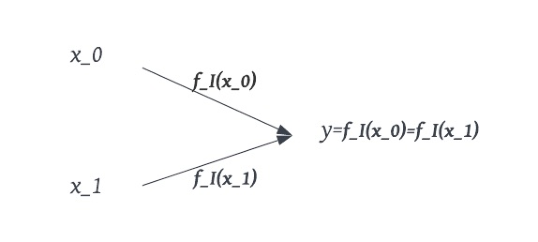
\includegraphics[]{figures/TCF.pdf}
	\caption{``A claw'' of a TCFs $f_{\mathcal{I}}(x)$ is a pair of $(x_0,x_1)$ such that $y=f_{\mathcal{I}}(x_0)=f_{\mathcal{I}}(x_1)$, $x_0\neq x_1$.}\label{fig:TCF}
\end{figure}


More formally, we can define the trapdoor claw-free function as follows:
\begin{Definition}[Trapdoor Claw-Free Function (TCFs)]
    Let $\mathcal{X}$, $\mathcal{Y}$ be finite sets, we require the family of functions $\mathcal{F}$ satisfies the following properties:
\begin{itemize}
    \item For each public key $k$ related to a problem instance $\mathcal{I}$, there are two functions $\{f_{\mathcal{I},b}:\mathcal{X}\to\mathcal{Y}\}_{b\in\{0,1\}}$ that are both injective and have the same range. These two functions are invertible given a suitable trapdoor $t_k$ (i.e.  $t_k$ can be used to efficiently compute $x$ given $b$ and $y=f_{\mathcal{I},b}(x)$). 
    \item The pair of functions should be \textit{claw-free}, i.e. it is hard to find the pair $(x_0,x_1)\in\mathcal{X}^2$ such that 
    \begin{align}
        y=f_{\mathcal{I},0}(x_0)=f_{\mathcal{I},1}(x_1) \text{ and } x_0\neq x_1.
        \label{eq:aclaw}
    \end{align}
\end{itemize}
\end{Definition}

\noindent Note that a quantum device cannot invert the function and find the claw $(x_0,x_1)$, but it can hold these two preimages together with $w$ in a superposition
\begin{align}
    \frac{1}{\sqrt{2}}(\ket{x_0}+\ket{x_1})\ket{w}.
    \label{eq:tcfstate1}
\end{align}
This is obtained by first preparing a uniform superposition over all $x\in\mathcal{X}$ via the Hadamard transform
\begin{align}
    \frac{1}{\sqrt{\mathcal{X}}}\sum_{x\in\mathcal{X}}\ket{x},
\end{align}
then evaluating $f_{\mathcal{I},b}(x)$ into an output register to yield 
\begin{align}
    \frac{1}{\sqrt{\mathcal{X}}}\sum_{x\in\mathcal{X}}\ket{x}\ket{f_{\mathcal{I},b}(x)}.\label{eq:tcfstate3}
\end{align}

When measuring the output register of the quantum state described by equation \eqref{eq:tcfstate3}, and obtaining a classical result $w$, the whole system undergoes a collapse, leading the state in the remaining register to collapse as well. The state would collapse to \eqref{eq:tcfstate1}, such that $w=f_{\mathcal{I},0}(x_0)=f_{\mathcal{I},1}(x_1)$. 

Measuring the~\eqref{eq:tcfstate1} state in the standard basis ($Z$ basis), one would obtain a random preimage as the measurement result, i.e. $m=x_0$ or $m = x_1$, but not both, since measuring a quantum state means collapsing that state to one possible outcome. Besides, measuring the~\eqref{eq:tcfstate1} state in the $X$ basis yields a measurement result $m$ and a bit $c$ that satisfies $m \cdot (x_0\oplus x_1) = c$. One may observe that the measurement result using the $X$ basis $(m,c)$ can be used as the hardcore bit, as in the case of a one-way function. However, there is a subtle point in using TCFs in cryptographic protocols: not all TCFs possess the hardcore bit property, just as not all one-way functions successfully hide the information of the input. In all existing TCFs constructions, the only one that satisfies the hardcore bit property is the one utilising LWE problem, we will go into more detail and explaination in the next subsection.

Note that these special properties of TCFs could be used to construct a Proof of Quantumness protocol, the details of which will be discussed in section~\ref{proof_of_quantumness}. However, a fully constructive TCFs that satisfies most cryptographic protocol requirements has not been explored yet. The paper \cite{Brakerski18_Interactiveproofofquantumness} considers a ``relaxed'' version of the TCFs, referred to as \textbf{Noisy trapdoor claw-free functions (NTCFs)}. For more detail and technical information about NTCFs, please refer to the Appendix~\ref{NTCFs}.

\subsection{TCFs from LWE}
\subsubsection{Definition}
For a matrix $\mathbf{A}\in\mathbb{Z}^{m\times n}_q$ and vectors $\mathbf{s}\in\{0,1\}^n$, $\mathbf{e}\in\{0,1\}^{m}$, consider the LWE instance $\mathcal{I}=(\mathbf{A},\mathbf{y}=\mathbf{A}\mathbf{s}+\mathbf{e})$ with the trapdoor $t_k=\{\mathbf{s},\mathbf{e}\}$. 

We can define the TCFs family  $\{f_{\mathcal{I},b}:\{0,1\}^n\to\mathbb{Z}^{m}\}_{b\in\{0,1\}}$ by letting 
\begin{align}
    f_{\mathcal{I},0}(\mathbf{x})=\mathbf{A}\mathbf{x}+\mathbf{e}_0\\
   f_{\mathcal{I},1}(\mathbf{x})=\mathbf{A}(\mathbf{x}+\mathbf{s})+\mathbf{e}_0+\mathbf{e}.
\end{align} 
If $\mathbf{e}_0 =\bf{0}$, the the claw are related by 
\begin{align}
    \mathbf{w}=f_{\mathcal{I},1}(\mathbf{x}_1)=f_{\mathcal{I},0}(\mathbf{x}_0)\\
    \mathbf{x}_1=\mathbf{x}_0-\mathbf{s}.\label{eq:preimages}
\end{align}
However, we need to hide the information of $\mathbf{x}$, it is essential to sample $\mathbf{e}_0$ from a Gaussian distribution much wider than $\mathbf{e}$ such that it ensures that the distribution of $f_{\mathcal{I},1}(\mathbf{x}_1)$ and $f_{\mathcal{I},0}(\mathbf{x}_0)$ are statistically close. This is why the construction of the paper~\cite{Brakerski18_Interactiveproofofquantumness} used the term ``noisy'' for its TCFs. For simplicity of our review, we will not dive into the details of NTCFs in the main sections and assume that one can efficiently find the claw $(\mathbf{x}_0,\mathbf{x}_1)$ satisfies ~\eqref{eq:preimages} using the trapdoor $t_k=\{\mathbf{s},\mathbf{e}\}$.



\subsubsection{Adaptive hardcore bit property for TCFs from LWE}

Recall that in the TCFs from LWE, measuring the output register of the~\eqref{eq:tcfstate3} state, obtaining the measurement outcome $\mathbf{w}$ and the superposition
\begin{align}
    \frac{1}{\sqrt{2}}(|\mathbf{x}_0\rangle +|\mathbf{x}_1\rangle)|\mathbf{w}\rangle.\label{eq:lwetfcstate}
\end{align}
\noindent Recall that when measuring the $\mathbf{x}$ register in the X basis, we obtain the measurement result $\mathbf{m}\in\{0,1\}^n$ and a bit $c\in\{0,1\}$ such that $\mathbf{m}\cdot(\mathbf{x}_0\oplus\mathbf{x}_1) = c$. This equation provides some information about both preimages. Consider the pre-images $\mathbf{x}_0$ and  $\mathbf{x}_1$ in~\eqref{eq:preimages}, we have that $\mathbf{s}$ is some fixed secret determined by the LWE problem instance $\mathcal{I}=(\mathbf{A},\mathbf{y}=\mathbf{A}\mathbf{s}+\mathbf{e})$. Hence, this equation can be rewritten as $\mathbf{m}'\cdot \mathbf{s} =c$. By repeating the entire procedure, one can have sufficient information about  $\mathbf{m}'$ to recover $\mathbf{s}$ with high probability. Hence, we need the structure of the function $f_{\mathcal{I},b}$ to be a little more complicated so that even knowledge about $(\mathbf{m},c)$, one cannot determine what the equation is about without additional knowledge of at least a preimage. As mentioned in the previous subsection, $\mathbf{m}\cdot(\mathbf{x}_0\oplus\mathbf{x}_1) = c$ can be use as hardcore bit that ensures it is ``hard'' to compute a bit of $\mathbf{x}_0$ or $\mathbf{x}_1$ given $\mathbf{w}$. Moreover, if an adversary can simultaneously find this predicate and a preimage $\mathbf{x}_b$, it could find the whole claw $(\mathbf{x}_0, \mathbf{x}_1)$.


%\noindent\textbf{Why does IPOF~\cite{Brakerski18_Interactiveproofofquantumness} construction use the term ``adaptive'' for the hardcore bits property?}

%Combining all the mentioned requirements, we can write the hardcore bit property for the LWE-based TCFs as follows:
%Given $f_{\mathcal{I},b}(\mathbf{x})$, a hardcore bit for $f$ is a $1$-output-bit function $h$ such that given  $f_{\mathcal{I},b}(\mathbf{x})$ (but not $\mathbf{x}$) it is hard to predict $h$. Here, the hardcore bit that underlies the assumption is the function $c = h(\mathbf{x})= \mathbf{m}\cdot (\mathbf{x}_0\oplus \mathbf{x}_1)$.
%

Moreover, we allow the adversary $\mathcal{A}$ to \textbf{\textit{adaptively choose the string $\mathbf{m}'$}}. This also means that more power is given to the adversary. It is in this sense that the hardcore bit property is \textbf{adaptive}. Concretely, in the LWE-based construction of~\cite{Brakerski18_Interactiveproofofquantumness}, the adversary $\mathcal{A}$ can adaptively choose the string $\mathbf{m}'$ after being given access to the LWE sample $(\mathbf{A},\mathbf{A}\mathbf{s}+\mathbf{e})$.
%, i.e. the choice of $\mathbf{m}'$ depend upon the LWE sample. 

Due to the \textit{leakage resilience} property of the LWE problem, the information of the $\mathbf{s}$ remains secret. The idea is that instead of sampling a uniformly random matrix $\mathbf{A}\in\mathbb{Z}^{m\times n}_q$ together with its trapdoor $\mathbf{s},\mathbf{e}$, we replace $\mathbf{A}$ by a ``lossy mode'' matrix $\tilde{\mathbf{A}}\in\mathbb{Z}^{m\times n}_q$, where $\tilde{\mathbf{A}}$ is sampled from a special distribution so that $\tilde{\mathbf{A}}=\mathbf{B}\mathbf{C}+\mathbf{E}$ for a skinny matrix $\mathbf{B}$, a wide matrix $\mathbf{C}$ and $\mathbf{E}\gets\mathcal{D}_{\mathbb{Z}_q}^{m\times n}$. It holds that $\tilde{\mathbf{A}}$ is indistinguishable from a uniformly random $\mathbf{A}$. Now, when we multiply $\tilde{\mathbf{A}}$ by $\mathbf{s}$, the matrix $\mathbf{C}$ compresses the information of $\mathbf{s}$. To be more specific, provided the matrix $\mathbf{C}$ is a uniformly random matrix with sufficiently few rows, the distribution $(\mathbf{C},\mathbf{C}\mathbf{s})$ for an arbitrary secret $\mathbf{s}$ does not reveal any parity of $\mathbf{s}$.
Hence, even having the power to adaptively repeat the process of choosing $\mathbf{m}'$, an adversary can not find $\mathbf{s}$ (or information of both preimages $\mathbf{x}_0$ and $\mathbf{x}_1$).
More information on the proof can be found in~\cite{Brakerski18_Interactiveproofofquantumness}.


\subsection{TCFs from RLWE}
Two years later from the first definition of the TCFs from LWE was published, Brakerski continued his work in~\cite{BrakerskiProofofQuantumness} and showed that using the ring version of the LWE problem yielded better results since RLWE-based primitives exhibit greater efficiency and yield smaller key sizes than their LWE-based counterparts, due to the ring dimension. This dimension plays a crucial role in determining the size of the challenge space. The larger the challenge space, the less the soundness error of the scheme has and the fewer times the underlying protocol has to repeat. 

Let $R_q=\mathbb{Z}[x]/(x^n+1)$, $\mathbf{a}$ is a vector of polynomials in $R_q^m$, $\mathbf{s}\in R_q$ and $\mathbf{e}$ is an error term sampled from a Discrete Gaussian distribution over $R_q$, consider the RLWE instance $\mathcal{I}=(\mathbf{a}\cdot s +\mathbf{e})$ with the trapdoor $t_k=(s,\mathbf{e})$.

The TCFs from RLWE problem can be defined as follows:
\begin{align}
    f_{\mathcal{I},0}(x)=\mathbf{a}\cdot x+\mathbf{e}_0,\\
    f_{\mathcal{I},1}(x)=\mathbf{a}\cdot (x+s)+\mathbf{e}_0+\mathbf{e},
\end{align}
where $\mathbf{e}_0$ is sampled from a wider Gaussian distribution compared to $\mathbf{e}$. 

Despite RLWE problems being considered more efficient than LWE problems, RLWE-based TCFs do not satisfy the adaptive hardcore bit property due to the absence of the lossiness argument in the RLWE problem. 
%%%%%%%%%%%%%%%%%%%%%%%%%%%%%%%%%%%%%%%%%%
\section{Proof of Quantumness} \label{proof_of_quantumness}

\subsection{Interactive proof}
A proof serves as a means of persuading someone that a specific statement is true. We typically involve two parties when discussing proofs: \textit{a prover} and \textit{a verifier}. The prover aims to convince the verifier of the validity of a given statement, while the verifier's goal is to accept only accurate arguments. Before defining the interactive proof, we first recall that a language is simply a set of strings $L\subseteq \{0,1\}^*$. The definition of an interactive proof for a statement $x$ in a language $L$ is defined as follows:

\begin{Definition}[Interactive proof]
    An interactive proof system for a language $L$ is a protocol between a computationally unrestricted prover $\mathcal{P}$ and a polynomial-time verifier $\mathcal{V}$ such that on input a statement $x$:
    \begin{itemize}
        \item \textbf{Completeness}: If $x\in L$, then an honest prover $\mathcal{P}$ that follows protocol should be able to convince the verifier $\mathcal{V}$ about the validity of the statement. 
        $$\forall x\in L, \Pr[(\mathcal{V}\leftrightarrow \mathcal{P})(x) \text{accepts }]=1.$$
        \item \textbf{Soundness $\epsilon$:} If $x \notin L$, then no malicious prover $\mathcal{P}'$ should be able to convince $\mathcal{V}$  with a success probability greater than $\epsilon$.
        $$\forall x\notin L, \forall \mathcal{P}', \Pr[(\mathcal{V}\leftrightarrow \mathcal{P}')(x) \text{accepts}]\leq \epsilon.$$
    \end{itemize}
\end{Definition}
\begin{figure}[!htb]
	\centering
	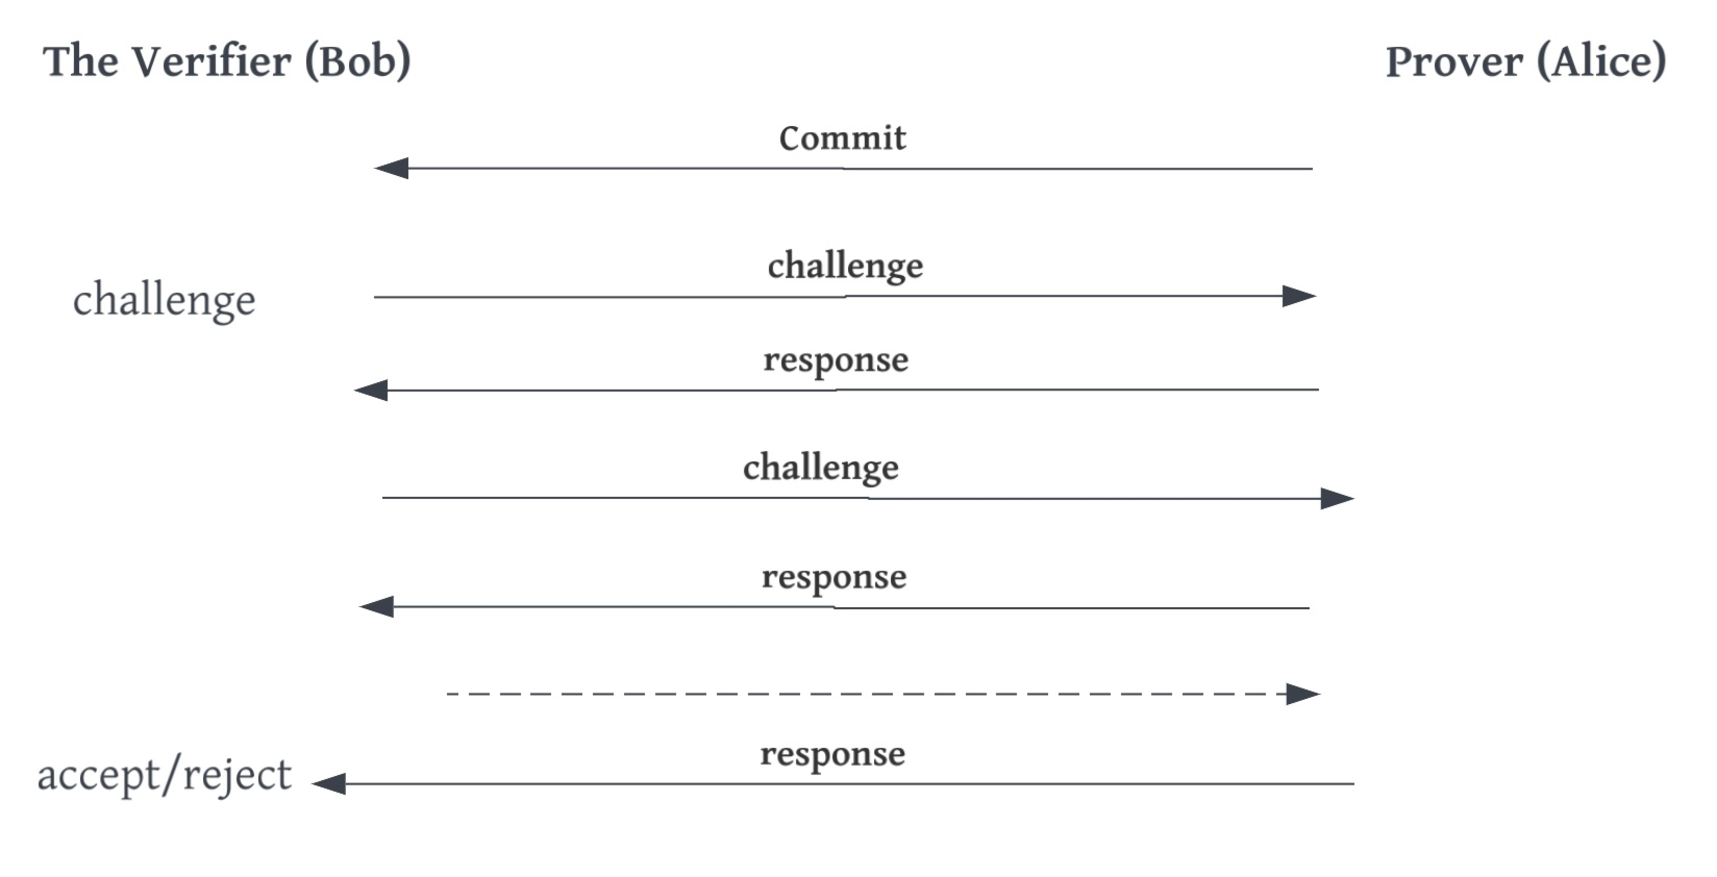
\includegraphics[scale = 0.35]{figures/IP.pdf}
	\caption{An interactive proof between a prover (Alice) and a verifier (Bob) typically has three main phases: commit, challenge, and response. The protocol may repeat the challenge-response phase multiple times to ensure the soundness property.}\label{fig:ip}
\end{figure}

\subsection{Proof of quantumness}
In recent years, under the efforts of building quantum computers, the verification of quantum behaviour has become significantly crucial. This underscores the necessity for a protocol in which a classical party can efficiently certify the quantum advantage of an untrusted device - the Proof of Quantumness. An interactive proof of quantumness~\cite{Brakerski18_Interactiveproofofquantumness,experiment_interactive_PoQ} is an interactive quantum verification protocol between two parties: a quantum prover $\mathcal{P}$ and a classical verifier $\mathcal{V}$. The verifier $\mathcal{V}$'s goal is to test the ``quantumness'' of the prover through an exchange of classical information. As mentioned in the end of the subsection~\ref{TCFs}, a common recent approach is to build the Interactive Proof of Quantumness protocol using TCFs.

%\begin{Definition}[Proof of Quantumness~\cite{liu22poqdefn}]
%     A proof of quantumness is an interactive protocol with an efficient classical verifier satisfying:
%     \begin{itemize}
%         \item \textbf{Completeness.} There exists a polynomial-time quantum prover that can convince the verifier about its ``quantum'' ability.
%         \item \textbf{Soundness} $\epsilon$.
%          Any polynomial-time classical prover convinces the verifier with probability at most $\epsilon + \mathsf{negl}$ for some negligible function $\mathsf{negl}$.
%     \end{itemize}
%\end{Definition}

\subsection{Interactive Proof of quantumness from LWE-based TFCs}
The basic idea of employing the TFCs from LWE to build the interactive proof of quantumness (IPQ) protocol is presented as follows:
\begin{enumerate}
    \item The verifier samples an LWE instance $\mathcal{I}=(\mathbf{A},\mathbf{y}=\mathbf{A}\mathbf{s}+\mathbf{e})$ together with a trapdoor $t_{k}=(\mathbf{s},\mathbf{e})$, and sends $\mathcal{I}$ and the description of the TCFs $f_{\mathcal{I},b}(\cdot)$ to the prover.
    \item The prover then:
    \begin{itemize}
        \item prepares a uniform superposition over $\mathbf{x}\in\{0,1\}^n$
        \begin{align}
            \frac{1}{\sqrt{2}^n}\sum_{\mathbf{x}\in\{0,1\}^n}\ket{\mathbf{x}},
        \end{align}
        \item evaluates $f_{\mathcal{I},b}(\cdot)$ into an output register yields the state
        \begin{align}
            \sum_{\mathbf{x}\in\{0,1\}^n}\ket{\mathbf{x}}\ket{f_{\mathcal{I},b}(\mathbf{x})},
        \end{align}        
        \item measures the output register to obtain $\mathbf{w}\in\mathcal{Y}$.
    The prover sends $\mathbf{w}$ to the verifier as the commitment for its quantum power.
    \end{itemize}
    \item The remaining state after measuring on the output register of the prover now is
    \begin{align}
        \frac{1}{\sqrt{2}}(\ket{\mathbf{x}_0}+\ket{\mathbf{x}_1})
    \end{align}
    where $\mathbf{x}_0$, $\mathbf{x}_1$ are two preimages of $\mathbf{w}$.
    \item The verifier challenges by asking the prover to measure on either the standard basis ($Z$ basis) ($\mathsf{chall}=0$) or the Hadamard basis ($X$ basis) ($\mathsf{chall}=1$).
    \item According to the verifier's challenge, the measurement outcome of the prover's state is:
    \begin{itemize}
        \item Standard basis: either $\mathbf{m}=\mathbf{x}_0$ or $\mathbf{m}=\mathbf{x}_1$, 
        \item Hadamard basis : $(\mathbf{m}\in\{0,1\}^n),c\in\{0,1\}$ such that $\mathbf{m}\cdot(\mathbf{x}_0\oplus\mathbf{x}_1)=c$.
    \end{itemize}
    \item The verifier checks these tests: 
    \begin{itemize}
        \item Standard basis: simply check that $f_{\mathcal{I},b}(\mathbf{m})=\mathbf{w}$.
        \item Hadamard basis: the verifier can recover $\mathbf{x}_0$, $\mathbf{x}_1$ from $\mathbf{y}$ using the trapdoor $t_k=(\mathbf{s},\mathbf{e})$, and check whether the pair $(\mathbf{m},c)$ satisfies $\mathbf{m}\cdot(\mathbf{x}_0+\mathbf{x}_1)=c$.
    \end{itemize}

The protocol proceeds for $\lambda$ rounds where $\lambda$ is the security parameter to ensure the soundness of the protocol. At the end of each round, the verifier samples a new problem instance and sends the new public key to the prover.
In a recent paper by Zhu~\cite{experiment_interactive_PoQ}, for each of the verifier’s possible choices, the experiment is repeated approximately $10^3$ times to collect statistics. 
\end{enumerate}

\begin{figure*}[!htp]
	\centering
	\begin{subfigure}[c]{\linewidth}
			\begin{quantikz}
\lstick{$f$} \setwiretype{c} & \gategroup[3,steps=7,style={rounded
    corners,fill=blue!10,draw=blue!50, inner
    xsep=5pt},background]{} & & & & \ctrl{0} & \setwiretype{n} & & & \lstick{$\mathsf{chall}$} & \setwiretype{c} \gategroup[3,steps=4,style={rounded
    corners,fill=blue!10,draw=blue!50, inner
    xsep=5pt},background]{} & & \ctrl{0} & \setwiretype{n} & \\
\setwiretype{n} & & \lstick{$\ket{\mathbf{0}}$} & \setwiretype{q} \qwbundle{n} & \gate{H^{\otimes n}} & \gate[2][5em]{U_f}\gateinput{$\mathbf{x}$}\gateoutput{$\mathbf{x}$}\wire[u]{c} & \qwbundle{n} & & & & & \qwbundle{n} & \gate{H^{\otimes n}}\wire[u]{c} & \meter{} & \setwiretype{c} \rstick{$\mathbf{m}$} & \setwiretype{n} & \\
\setwiretype{n} & & \lstick{$\ket{\mathbf{0}}$} & \setwiretype{q} \qwbundle{n-1} & & \gateinput{$\mathbf{y}$}\gateoutput{$\mathbf{y}\oplus f(x)$} & \qwbundle{n-1} & \meter{} & \setwiretype{c} \rstick{$\mathbf{w}$} & \setwiretype{n} & & & & & &
\end{quantikz}

			\caption{The IPQ protocol, where $f$ is the TCFs chosen by the verifier. The prover executes the first round of the protocol, measuring the output register to obtain classical outcome $\mathbf{w}$. After receiving $\mathbf{w}$ from the prover the verifier communicates a random measurement basis $Z$ or $X$ by sending a bit ($\mathsf{chall}\in\{0,1\}$) for the prover to measure the $\mathbf{x}$ register (the random challenge). This process yields an outcome $\mathbf{m}\in\{0,1\}^n$. Knowing the secret trapdoor, the verifier can efficiently verify the prover's response.}
	\end{subfigure}\label{fig:ipqlwe}
 \\
	\begin{subfigure}[c]{\linewidth}
		\begin{quantikz}
\lstick{$f$} \setwiretype{c} & \gategroup[3,steps=9,style={rounded
    corners,fill=blue!10,draw=blue!50, inner
    xsep=5pt},background]{} & & & & \ctrl{0} & \setwiretype{n} & & & & \\
\setwiretype{n} & & \lstick{$\ket{\mathbf{0}}$} & \setwiretype{q} \qwbundle{n} & \gate{H^{\otimes n}} & \gate[2][5em]{U_f}\gateinput{$x$}\gateoutput{$x$}\wire[u]{c} &\qwbundle{n} & \gate{U_h} & \gate{H^{\otimes n}} & \meter{} & \setwiretype{c} \rstick{$\mathbf{m}$} & \setwiretype{n} & \\
\setwiretype{n} & & \lstick{$\ket{\mathbf{0}}$} & \setwiretype{q} \qwbundle{n-1} & & \gateinput{$\mathbf{y}$}\gateoutput{$\mathbf{y}\oplus f(x)$} & \qwbundle{n-1} & \phantomgate{U_h} & \phantomgate{H^{\otimes n}} & \meter{} & \setwiretype{c} \rstick{$\mathbf{w}$} & \setwiretype{n} &
\end{quantikz}

		\caption{Non-interactive PQ protocol, replacing the randomly chosen challenge $\mathsf{chall}\in\{0,1\}$ by using a hash-function-based quantum random oracle.}
	\end{subfigure}\label{fig:ipqrlwe}
	\caption{\textbf{Quantum circuits for proofs-of-quantumness protocols.} \\Blue boxes contain all quantum operations within the protocol with classical inputs and outputs.} \label{fig:IPQ_circuit.tex}
\end{figure*}

\noindent\textbf{Analysis.} For the proof of quantumness protocol, the post-quantum cryptography hardness assumption here is employed in a different way, where we do not require the prover to break something that the classical machine cannot. The protocol is constructed in a way that the security is preserved even against both \textit{classical} and \textit{quantum} prover. We use the \textit{rewinding} technique to distinguish between the classical and quantum cases. If a classical prover can cause the verifier to accept the statement, it can rewind and thus break the underlying hardness assumption which is computationally infeasible due to the hardness of the LWE problem. However, if the prover is ``quantum,'' it can persist with the verifier without breaking the underlying cryptographic assumption while performing measurements that cannot be reversed due to the no-cloning theorem.

Note the adaptive hardcore bit property plays an important role in this IPQ construction. Suppose there exists a prover capable of successfully navigating both verifier challenges. Specifically, given the problem instance $\mathcal{I}$, this prover can generate a tuple $(\mathbf{w}, b, \mathbf{x}_b, (\mathbf{m}, c))$ with $b,c \in {0,1}$ that satisfies two checks with a probability significantly higher than $1/2$, i.e., $f_{\mathcal{I},b}(\mathbf{x}_b) = \mathbf{w}$, $\mathbf{m} \cdot (\mathbf{x}_0 \oplus \mathbf{x}_1) = c$, and $\mathbf{m} \neq \mathbf{0}^n$.
It is important to note that in this scenario, the prover does not discover the entire claw $(\mathbf{x}_0, \mathbf{x}_1)$ but rather identifies one preimage $\mathbf{x}_b$ along with a linear function of the other preimage $\mathbf{x}_{1-b}$. Therefore, the \textbf{hardcore bit} property is indispensable, asserting that it is computationally challenging to find even a single bit of $\mathbf{x}_{1-b}$—meaning the prover cannot determine a single bit of $\mathbf{x}_{1-b}$, let alone the entire claw. 


\subsection{Non-interactive proof of quantumness from the RLWE problem}

Recall that up till now, the hardcore bit property has only been shown for TCFs based on the LWE problem. However, it is still possible to construct a \textbf{non-interactive proof of quantumness} protocol based on other hardness assumptions. \cite{BrakerskiProofofQuantumness} employs the \textbf{random oracle heuristic} as a tool to reduce the round complexity of the proof of quantumness protocol which also makes it possible to implement the protocol in a single round and eliminates the need for the hard-core bit property. The quantum device must evaluate the random oracle on a quantum superposition.

Assume we have a hash function $h(\cdot)$. In the unitary model of quantum computing, consider this means that there exists a unitary $U_h$ that performs the mapping 
$$U_h: \ket{\mathbf{x}}\ket{\mathbf{y}} \mapsto \ket{\mathbf{x}}\ket{\mathbf{x}\oplus h(\mathbf{x})}$$
on the basis states.

%For an element $\mathbf{x}$, $\mathsf{BitDecomp}(\mathbf{x})$ is the binary representation of $\mathbf{x}$. 
The proof of quantumness protocol is now parameterised by a hash function $h:\{0,1\}^n\to\{0,1\}$ as follows:
\begin{enumerate}
    \item The verifier generates a problem instance $\mathcal{I}$ and trapdoor $t_k$ and sends $\mathcal{I}$ to the prover.
    \item The prover sends $\lambda$ tuple $\{(\mathbf{w}_i,c_i,\mathbf{m}_i)\}_{i\in[\lambda]}$, where $\lambda$ is the security parameter. The verifier initialises $\mathsf{count}=0$ and performs the following checks:
    \begin{itemize}
        \item It checks that all value $\{\mathbf{w}_i\}_{i\in[\lambda]}$ are distinct.
        \item It uses the trapdoor to compute $\mathbf{x}_{i,b}$ for each $i\in[\lambda]$ and $b\in\{0,1\}$. The verifier then checks 
        %$c_i=\mathbf{m}_i^T\cdot(\mathsf{BitDecomp}(x_{i,0})+\mathsf{BitDecomp}(x_{i,1}))+h(x_{i,0})+h(x_{i,1})$. If $(c_i,d_i)$ 
        $c_i=\mathbf{m}_i\cdot(\mathbf{x}_{i,0}\oplus\mathbf{x}_{i,1})\oplus h(\mathbf{x}_{i,0})\oplus h(\mathbf{x}_{i,1})$. 
        If $(c_i,\mathbf{m}_i)$
        satisfies this equation, it increases the value of $\mathsf{count}$ by $1$.
    \end{itemize}
    \item If $\mathsf{count}>0.75\lambda$, the verifier accepts, else it rejects.
\end{enumerate}

The second figure in Figure~\ref{fig:IPQ_circuit.tex} represents the non-interactive proof of quantumness, which removes the interaction between the prover and the verifier during the challenge phase using the hash function $h(\cdot)$, as demonstrated above. Using the RLWE problem, we can significantly reduce the size of keys and the commitment of the construction.  

\textbf{Why can using the hash function can replace the hardcore bit property?} Recall that in the LWE-based proof of quantumness construction~\cite{Brakerski18_Interactiveproofofquantumness}, the prover applies the TCFs $f_{\mathcal{I},b}(\mathbf{x})$ on a uniform superposition of inputs and then measures the image register. It then obtains the value $\mathbf{w}$, which will be sent to the verifier. The prover now has a state that is a superposition over $\mathbf{x}_0$ and $\mathbf{x}_1$. The prover then has to measure this state according to the challenge of the verifier: measure using the standard basis or Hadamard basis. A malicious prover that can break the protocol must be able to answer both challenges by the verifier simultaneously, which violates the \textit{hardcore bit property} and the hardness assumption. Using a one-bit hash function $h(\mathbf{x}):\{0,1\}^n\to \{0,1\}$,~\cite{BrakerskiProofofQuantumness} generates the superposition over $(0,\mathbf{x}_0,h(\mathbf{x}_0))$ and $(1,\mathbf{x}_1,h(\mathbf{x}_1))$. The prover is then asked to measure the resulting state on a Hadamard basis only and send the outcome to the verifier, including a bit $c$ and the measurement outcome $\mathbf{m}$. It holds that $(c,\mathbf{m})$ satisfies the hardcore predicate $c=\mathbf{m}\cdot(\mathbf{x}_0\oplus \mathbf{x}_1)\oplus h(\mathbf{x}_0)\oplus h(\mathbf{x}_1)$. The verifier employs the trapdoor to recover $(\mathbf{w},\mathbf{x}_0,\mathbf{x}_1)$ and verifies whether the above equation is satisfied. The security of the protocol is upheld because an adversary cannot query the random oracle for both $\mathbf{x}_0$ and $\mathbf{x}_1$; thus, at least one value $h(\mathbf{x}_0)$ or $h(\mathbf{x}_1)$ remains random. This implies the malicious prover cannot compute $(c,\mathbf{x})$ satisfying the equation with a probability greater than $1/2$. Consequently, this also eliminates the need for the hardcore bit property. 

\section{Comparison on experimental results}

This section gives the connection between result measurements in the original and experimental papers.

\begin{table}[!htp] 
\caption{Comparison between the Proof of Quantumness protocols.\label{t_2}\label{tab:compare}}
\begin{tabularx}{\textwidth}{CCCCCCC}
\toprule
\textbf{Paper}	& \textbf{Problem}	& \textbf{Adaptive hardcore bit} &\textbf{Interactive}&\textbf{Using hash function}&\textbf{Gate count}&\textbf{Adversary type}\\
\midrule
\cite{Brakerski18_Interactiveproofofquantumness} & LWE	& \cmark & \cmark & \xmark & $n^2\log^2n$ & classical\\
\cite{experiment_interactive_PoQ} & LWE	& \cmark & \cmark & \xmark & $n^2\log^2n$ & classical\\
\cite{BrakerskiProofofQuantumness} & RLWE & \xmark & \xmark & \cmark & $n\log^2n$ & quantum\\
\cite{experiment_non_interactive_PoQ} & RLWE & \xmark & \xmark & \cmark & $n\log^2n$ & quantum\\
\bottomrule
\end{tabularx}
\end{table}


%%%%%%%%%%%%%%%%%%%%%%%%%%%%%%%%%%%%%%%%%%
\section{Discussion}


%%%%%%%%%%%%%%%%%%%%%%%%%%%%%%%%%%%%%%%%%%
\section{Conclusions}




%%%%%%%%%%%%%%%%%%%%%%%%%%%%%%%%%%%%%%%%%%
\vspace{6pt} 

%%%%%%%%%%%%%%%%%%%%%%%%%%%%%%%%%%%%%%%%%%
%% optional
%\supplementary{The following supporting information can be downloaded at:  \linksupplementary{s1}, Figure S1: title; Table S1: title; Video S1: title.}

% Only for journal Methods and Protocols:
% If you wish to submit a video article, please do so with any other supplementary material.
% \supplementary{The following supporting information can be downloaded at: \linksupplementary{s1}, Figure S1: title; Table S1: title; Video S1: title. A supporting video article is available at doi: link.}

% Only for journal Hardware:
% If you wish to submit a video article, please do so with any other supplementary material.
% \supplementary{The following supporting information can be downloaded at: \linksupplementary{s1}, Figure S1: title; Table S1: title; Video S1: title.\vspace{6pt}\\
%\begin{tabularx}{\textwidth}{lll}
%\toprule
%\textbf{Name} & \textbf{Type} & \textbf{Description} \\
%\midrule
%S1 & Python script (.py) & Script of python source code used in XX \\
%S2 & Text (.txt) & Script of modelling code used to make Figure X \\
%S3 & Text (.txt) & Raw data from experiment X \\
%S4 & Video (.mp4) & Video demonstrating the hardware in use \\
%... & ... & ... \\
%\bottomrule
%\end{tabularx}
%}

%%%%%%%%%%%%%%%%%%%%%%%%%%%%%%%%%%%%%%%%%%
\authorcontributions{For research articles with several authors, a short paragraph specifying their individual contributions must be provided. The following statements should be used ``Conceptualization, X.X. and Y.Y.; methodology, X.X.; software, X.X.; validation, X.X., Y.Y. and Z.Z.; formal analysis, X.X.; investigation, X.X.; resources, X.X.; data curation, X.X.; writing---original draft preparation, X.X.; writing---review and editing, X.X.; visualization, X.X.; supervision, X.X.; project administration, X.X.; funding acquisition, Y.Y. All authors have read and agreed to the published version of the manuscript.'', please turn to the  \href{http://img.mdpi.org/data/contributor-role-instruction.pdf}{CRediT taxonomy} for the term explanation. Authorship must be limited to those who have contributed substantially to the work~reported.}

\funding{Please add: ``This research received no external funding'' or ``This research was funded by NAME OF FUNDER grant number XXX.'' and  and ``The APC was funded by XXX''. Check carefully that the details given are accurate and use the standard spelling of funding agency names at \url{https://search.crossref.org/funding}, any errors may affect your future funding.}

\institutionalreview{In this section, you should add the Institutional Review Board Statement and approval number, if relevant to your study. You might choose to exclude this statement if the study did not require ethical approval. Please note that the Editorial Office might ask you for further information. Please add “The study was conducted in accordance with the Declaration of Helsinki, and approved by the Institutional Review Board (or Ethics Committee) of NAME OF INSTITUTE (protocol code XXX and date of approval).” for studies involving humans. OR “The animal study protocol was approved by the Institutional Review Board (or Ethics Committee) of NAME OF INSTITUTE (protocol code XXX and date of approval).” for studies involving animals. OR “Ethical review and approval were waived for this study due to REASON (please provide a detailed justification).” OR “Not applicable” for studies not involving humans or animals.}

\informedconsent{Any research article describing a study involving humans should contain this statement. Please add ``Informed consent was obtained from all subjects involved in the study.'' OR ``Patient consent was waived due to REASON (please provide a detailed justification).'' OR ``Not applicable'' for studies not involving humans. You might also choose to exclude this statement if the study did not involve humans.

Written informed consent for publication must be obtained from participating patients who can be identified (including by the patients themselves). Please state ``Written informed consent has been obtained from the patient(s) to publish this paper'' if applicable.}

\dataavailability{We encourage all authors of articles published in MDPI journals to share their research data. In this section, please provide details regarding where data supporting reported results can be found, including links to publicly archived datasets analyzed or generated during the study. Where no new data were created, or where data is unavailable due to privacy or ethical restrictions, a statement is still required. Suggested Data Availability Statements are available in section ``MDPI Research Data Policies'' at \url{https://www.mdpi.com/ethics}.} 

% Only for journal Nursing Reports
%\publicinvolvement{Please describe how the public (patients, consumers, carers) were involved in the research. Consider reporting against the GRIPP2 (Guidance for Reporting Involvement of Patients and the Public) checklist. If the public were not involved in any aspect of the research add: ``No public involvement in any aspect of this research''.}

% Only for journal Nursing Reports
%\guidelinesstandards{Please add a statement indicating which reporting guideline was used when drafting the report. For example, ``This manuscript was drafted against the XXX (the full name of reporting guidelines and citation) for XXX (type of research) research''. A complete list of reporting guidelines can be accessed via the equator network: \url{https://www.equator-network.org/}.}

% Only for journal Nursing Reports
%\useofartificialintelligence{Please describe in detail any and all uses of artificial intelligence (AI) or AI-assisted tools used in the preparation of the manuscript. This may include, but is not limited to, language translation, language editing and grammar, or generating text. Alternatively, please state that “AI or AI-assisted tools were not used in drafting any aspect of this manuscript”.}

\acknowledgments{In this section you can acknowledge any support given which is not covered by the author contribution or funding sections. This may include administrative and technical support, or donations in kind (e.g., materials used for experiments).}

\conflictsofinterest{Declare conflicts of interest or state ``The authors declare no conflicts of interest.'' Authors must identify and declare any personal circumstances or interest that may be perceived as inappropriately influencing the representation or interpretation of reported research results. Any role of the funders in the design of the study; in the collection, analyses or interpretation of data; in the writing of the manuscript; or in the decision to publish the results must be declared in this section. If there is no role, please state ``The funders had no role in the design of the study; in the collection, analyses, or interpretation of data; in the writing of the manuscript; or in the decision to publish the results''.} 

%%%%%%%%%%%%%%%%%%%%%%%%%%%%%%%%%%%%%%%%%%
%% Optional

%% Only for journal Encyclopedia
%\entrylink{The Link to this entry published on the encyclopedia platform.}

\abbreviations{Abbreviations}{
The following abbreviations are used in this manuscript:\\

\noindent 
\begin{tabular}{@{}ll}
PQC & Post-quantum cryptography\\
RSA & Rivest-Shamir-Adleman algorithm\\
ECC & Elliptic curve cryptography\\
QKD & Quantum key distribution\\
IPQ & Interactive proof of quantumness\\
SVP & Shortest vector problem\\
SIVP & Shortest independent vectors problem\\
CVP & Closest vector problem\\
SIS & Short integer solution\\
LWE & Learning with error\\
RLWE & Ring-Learning with error\\
TFCs & Trapdoor claw-free functions\\
NTCFs & Noisy trapdoor claw-free functions
\end{tabular}
}

%%%%%%%%%%%%%%%%%%%%%%%%%%%%%%%%%%%%%%%%%%
%% Optional
\appendixtitles{no} % Leave argument "no" if all appendix headings stay EMPTY (then no dot is printed after "Appendix A"). If the appendix sections contain a heading then change the argument to "yes".
\appendixstart
\appendix
\section[\appendixname~\thesection]{Ring Learning With Errors problem (RLWE)}~\label{RLWE}

Here, let's first recall some basic ideas of the RLWE problem.

\subsubsection{The initial idea.}
Let's recall that the SIS problem in Eq.~\eqref{eq:linear_equation} yields a very simple collision-resistant hash function that is provably secure if worst-case lattice problems are hard:
\begin{align}
    h_{\mathbf{A}}(\mathbf{s})=\mathbf{A}\mathbf{s} \mod q
\end{align}
where $\mathbf{A}\in\mathbb{Z}^{m\times n}_q$ is uniformly random and $\mathbf{s}\in \{0,1\}^n$. 

However, this is inefficient, since just reading the public description of $\mathbf{A}$ takes time roughly $mn\log q>n^2$. The goal is now to show a variant of $h_{\mathbf{A}}$ whose running time is roughly linear in $n$. 

A trivial idea is taking some short, uniformly random seed $r$ and then setting $\mathbf{A} = H(\textsf{seed})$ for some suitable expanding function $H$. However, we need to describe $H$ so that it can be efficiently used in cryptography constructions. 


Let's first take the random seed to be $\ell = m/n$ uniformly random vectors $\mathbf{a}_1,\dots,\bf{a_{\ell}}\in[q]^n$. Consider the ``cyclic rotations'' of $\mathbf{a}_i$, i.e. for a single vector $\mathbf{a}=(a_1,\dots,a_n)^T\in\mathbb{Z}^n$, we define
\begin{align}
    \mathsf{Rot}(\mathbf{a})=
    \begin{pmatrix}
    a_1 & a_n &\dots& a_3 & a_2\\
    a_2 & a_n &\dots& a_4 & a_3\\
    a_3 & a_n &\dots& a_5 & a_4\\
    \vdots & \vdots &\ddots& \vdots & \vdots\\
    a_{n-2} & a_{n-3} &\dots& a_n & a_{n-1}\\
    a_{n-1} & a_{n-2} &\dots& a_1 & a_n\\
    a_{n} & a_{n-1} &\dots& a_2 & a_1
    \end{pmatrix}\in\mathbb{Z}^{n\times n},
\end{align}
    where each column is a simple cyclic permutation of the previous column. 
    %Matrices of the form $\mathsf{Rot}(\mathbf{a})$ are sometimes called \textit{cyclic matrices}. 
    $\mathbf{A}$ can now be rewritten as
\begin{align}
    \mathbf{A}=
    \begin{pmatrix}
    \mathsf{Rot}(\mathbf{a}_1)\\
    \mathsf{Rot}(\mathbf{a}_2)\\
    \vdots\\
    \mathsf{Rot}(\mathbf{a}_{\ell})
    \end{pmatrix}\in\mathbb{Z}^{m\times n}.
\end{align}

\noindent Due to the property of $\mathsf{Rot}(\mathbf{a}$, we can write $\mathsf{Rot}(\mathbf{a})=(\mathbf{a}),\bf{X}\mathbf{a},\dots,X^{n-1}\mathbf{a})$ 
where 
\begin{align}
    \bf{X}=
    \begin{pmatrix}
    0 & 0 &\dots& 0 & 1\\
    1 & 0 &\dots& 0 & 0\\
    0 & 1 &\dots& 0 & 0\\
    \vdots & \vdots &\ddots& \vdots & \vdots\\
    0 & 0 &\dots& 1 & 0
    \end{pmatrix}\in\{0,1\}^{n\times n}
\end{align}
    is the ``cyclic shift'' matrix. 
   
\noindent Consider the set of all integer cyclic matrices, $\Tilde{R}:=\{\mathsf{Rot}(\mathbf{a}):\mathbf{a}\in\mathbb{Z}^n\}$. Hence we have that $\Tilde{R}$ is a lattice with rank $n$ and basis $\{\bf{I}_n,\bf{X},\bf{X}^2,\dots,\bf{X}^{n-1}\}$. We have that $\tilde{R}$ is a commutative ring. We can instead think of $\mathsf{Rot}(\mathbf{a})\in\tilde{R}$ as the corresponding polynomial $a\in R=\mathbb{Z}[x]/(x^n-1)$. Hence, we can therefore identify the matrix $\mathbf{A}\in\mathbb{Z}_q^{m \times n}$ with a tuple of ring elements $(a_1,\dots,a_{\ell})^T\in R^{\ell}_q= R=\mathbb{Z}^{\ell}_q[x]/(x^n-1)$. Similarly, $\mathbf{s}$ is a tuple of ring elements $(s_1,\dots,s_{\ell})^T\in R^{\ell}_{\{0,1\}}$.
    Therefore, $h_{\mathbf{A}}$ can be written as 
\begin{align}
    h_a(s)=h_{a_1,\dots,a_{\ell}}(s_1,\dots,s_{\ell})=a_1s_1+\dots+s_{\ell}s_{\ell}\mod qR.
\end{align}
     The Ring-SIS problem, which is the analogue of SIS in this setting, can be defined as follows: For a ring $R$, integer modulus $q\geq 2$, and integer $\ell\geq 1$. Given $a_1,\dots, a_{\ell}\in R_q$ sampled independently and uniformly at random. The search Ring-SIS problem asks to output $e_1,\dots e_{\ell}\in R_{\{-1,0,1\}}$ not all zero such that $h_{a_1,\dots,a_{\ell}}(e_1,\dots,e_{\ell})=a_1e_1+\dots+a_{\ell}e_{\ell} = 0\mod qR$.


    However, for security reasons, there exist attacks on $h_a$ over $\mathbb{Z}[x]/(x^n-1)$ since $(x^n-1)$ has a nontrivial factor over the integers. So, it is natural to try replacing $(x^n-1)$ with an irreducible polynomial $p(x)$. 


    If $n$ is a power of $2$, we have that $x^n+1$ is an irreducible polynomial and $R=\mathbb{Z}[x]/(x^n+1)$ is an integral domain. From the matrix perspective mentioned above, this corresponds to taking
\begin{align}
    \mathsf{Rot}(\mathbf{a})=
    \begin{pmatrix}
    a_1 & -a_n &\dots& -a_3 & -a_2\\
    a_2 & a_n &\dots& -a_4 & -a_3\\
    a_3 & a_n &\dots& -a_5 & -a_4\\
    \vdots & \vdots &\ddots& \vdots & \vdots\\
    a_{n-2} & a_{n-3} &\dots& -a_n & -a_{n-1}\\
    a_{n-1} & a_{n-2} &\dots& -a_1 & -a_n\\
    a_{n} & a_{n-1} &\dots& a_2 & a_1
    \end{pmatrix}\in\mathbb{Z}^{n\times n},
\end{align}
    and 
\begin{align}
    \bf{X}=
    \begin{pmatrix}
    0 & 0 &\dots& 0 & -1\\
    1 & 0 &\dots& 0 & 0\\
    0 & 1 &\dots& 0 & 0\\
    \vdots & \vdots &\ddots& \vdots & \vdots\\
    0 & 0 &\dots& 1 & 0
    \end{pmatrix}\in\{-1,0,1\}^{n\times n}.
\end{align}
    Matrices of the form $\mathsf{Rot}(\mathbf{a})$ as above are occasionally called ``\textit{anti-cyclic}''. Ring-SIS is hard over this ring, under a reasonable worst-case complexity assumption.

\subsubsection{Ideal lattices and computational problems}
Recall that a lattice is an additive subgroup of $\mathbb{Z}^n$,i.e., a subset of $\mathbb{Z}^n$ closed under addition and subtraction. An ideal $\mathcal{I}\subset R=\mathbb{Z}[x]/(x^n+1)$ is an additive subgroup of $R$ that is closed under multiplication by any ring element. Concretely, $\mathcal{I}$ is closed under addition and subtraction, and for any $y\in\mathcal{Y}$ and $r\in R$, we have that $ry\in\mathcal{I}$.

For the choice of ring, we can view $\mathcal{I}$ as a lattice by embedding $R$ in $\mathbb{Z}^n$ via the trivial embedding that maps $x_i$ to the unit vector $\mathbf{e}_i$. We have that $\mathcal{I}\subset \mathbb{Z}^n$ is a lattice such that $(y_1,\dots,y_n)^T \in \mathcal{I}$ if and only if $(-y_n,y_1\dots,y_{n-1})^T \in \mathcal{I}$. Such lattices are sometimes called ``anti-cyclic" lattices.\\
This view of ideals as lattices is useful since we can extend computational lattice problems to ideals. Concretely, for some fixed ring $R$, we can define the computational problems IdealSVP, IdealSIVP, GapIdealSVP, etc., similar to SVP, SIVP, etc. as the corresponding computational problems restricted to ideal lattices.

\section[\appendixname~\thesection]{Noisy Trapdoor Claw-free Functions (NTCFs)}~\label{NTCFs}
In NTCFs, the range of functions $f_{k,0}$ and $f_{k,1}$ is represented by a distribution $\mathcal{D}$ over $\mathcal{Y}$, denoted as $\mathcal{D}_{\mathcal{Y}}$. In other words, each function returns a density rather than a point. Instead of considering the range of $f{k,b}$, we consider the support of the output densities, $\mathsf{SUPP}(f_{\mathcal{I},b}(x))$. If $y$ lies in this support, a party that holds the trapdoor $t_k$ can use it to invert the function and find the preimages of $y$.

\begin{Definition}[Noisy Trapdoor Claw-Free family]
   Let $\lambda$ be a security parameter. Let $\mathcal{X}$ and $\mathcal{Y}$ be finite sets. Let $\mathcal{K}_{\mathcal{F}}$ be a finite set of keys. A family of functions
   \begin{align}
       \mathcal{F}=\{f_{\mathcal{I},b}:\mathcal{X}\to \mathcal{D}_{\mathcal{Y}}\}_{b\in\{0,1\}}
   \end{align}
is called a noisy trapdoor claw-free (NTCF) family if the following conditions hold:
\begin{enumerate}
    \item \textbf{Efficient Function Generation.} There exists an efficient probabilistic algorithm $\mathsf{GEN}_{\mathcal{F}}$ which generates problem instance $\mathcal{I}$ together with a trapdoor $t_{k}$:
    \begin{align}
        \mathsf{GEN}_{\mathcal{F}}(1^{\lambda})\to (\mathcal{I},t_k).
    \end{align}
    \item \textbf{Trapdoor Injective Pair.}
    \begin{itemize}
        \item \textit{Trapdoor:} There exists an efficient deterministic algorithm \textit{Invert} $\mathsf{INV}_\mathcal{F}$ such that with overwhelming probability over the choice of $(\mathcal{I},t_k)$, the following holds:
        \begin{center}
            for all $b\in\{0,1\}$, $\mathbf{x}\in \mathcal{X}$ and $y\in \mathsf{SUPP}(f_{\mathcal{I},b}(x))$, $\mathsf{INV}_\mathcal{F}(t_k,b,y)=x$.
        \end{center}
        \item \textit{Injective pair:} There exists a perfect matching set for an instance $\mathcal{I}$ denoted  $\mathcal{R}_{\mathcal{I}}\subseteq \mathcal{X}\times \mathcal{X}$ such that $f_{\mathcal{I},0}(x_0)=f_{\mathcal{I},0}(x_1)$ if and only if $(x_0,x_1)\in \mathcal{R}_{\mathcal{I}}$. 
    \end{itemize}
    \item \textbf{Efficient Range Superposition.} For all keys $k\in \mathcal{K}_{\mathcal{F}}$ and $b\in\{0,1\}$ there exists a function $f'_{\mathcal{I},b}:\mathcal{X}\to \mathcal{D}_{\mathcal{Y}}$ such that the following hold:
    \begin{itemize}
        \item For all $(x_0,x_1)\in \mathcal{R}_k$ and $y\in\mathsf{SUPP}(f'_{\mathcal{I},b})(x_b)$, $\mathsf{INV}_{\mathcal{F}}(t_k,b\oplus 1,y)=x_{x\oplus 1}$.
        \item There exists an efficient deterministic procedure $\mathsf{CHK}_{\mathcal{F}}$ that given set of input $\mathcal{I}$, $b\in\{0,1\}$, $x\in \mathcal{X}$ and $y\in \mathcal{Y}$, check whether $y$ is an element of the support of $f$ or not. This procedure returns $1$ if $y\in \mathsf{SUPP}(f'_{\mathcal{I},b}(x))$ and $0$ otherwise. 
        %Note that $\mathsf{CHK}_{\mathcal{F}}$ is not provided the trapdoor $t_{k}$.
        \item 
        %For every $k$ and $b\in\{0,1\}$,
        %$$E_{x\gets_U \mathcal{X}}[H^2(f_{\mathcal{I},b}(x),f'_{k,b}(x))]\leq 1/50.$$
        %Here $H^2$ is the Hellinger distance. Moreover, 
        There exists an efficient procedure $\mathsf{SAMP}_{\mathcal{F}}$ that on input the problem instance $\mathcal{I}$ and $b\in\{0,1\}$, prepares the state
        \begin{align}
            \displaystyle{\frac{1}{\sqrt{|\mathcal{X}|}}}\sum_{x\in\mathcal{X},y\in\mathcal{Y}}\sqrt{(f'_{\mathcal{I},b}(x)(y))}|x\rangle|y\rangle.
        \end{align}
    \end{itemize}
    \item \textbf{Claw-free Property.} There no probabilistic polynomial time adversary $\mathcal{A}$ can find the ``claw'' $(x_0,x_1,y)$. More formally, there exists a negligible function $\mathsf{negl}(\cdot)$ such that the following holds:
    \begin{align}
        \Pr[(x_0,x_1)\in\mathcal{R}_{\mathcal{I}}:(\mathcal{I},t_k)\gets \mathsf{GEN}_{\mathsf{F}}(1^{\lambda}),(x_0,x_1)\gets \mathcal{A}(\mathcal{I)}]\leq \mathsf{negl}(\lambda).
    \end{align}
\end{enumerate}
\end{Definition}
\subsection[\appendixname~\thesubsection]{NTCFs from LWE}
\cite{Brakerski18_Interactiveproofofquantumness} built a NTCFs family from the LWE problem as follows:

\begin{Definition}[NTCFs based on LWE~\cite{Brakerski18_Interactiveproofofquantumness}\label{defn:tcfsfromlwe}]
    Let $\lambda$ be a security parameter. Let $q\geq 2$ be a prime and $\ell,n,m\geq 1$ are polynomially bounded functions of $\lambda$, and $B_L,B_V, B_P$ be positive integers such that the following conditions hold:
    \begin{itemize}
        \item $n=\Omega(\ell\log q +\lambda)$,
        \item $m=\Omega(n\log q)$,
        \item $B_P = \displaystyle{\frac{q}{2C_T\sqrt{mn\log q}}}$, for $C_T$ is a universal constant in the $\mathsf{GenTrap}$ algorithm.
    %\item We have $B_L<B_V<B_P$ so that the ratios $\frac{B_P}{B_V}$ and $\frac{B_V}{B_L}$ are both super-polynomial in $\lambda$.
    \end{itemize}
\begin{enumerate}
    \item \textbf{Efficient Function Generation:} The $\mathsf{GEN}_{\mathcal{F}}(1^{\lambda})$ is constructed as follows:
    \begin{itemize}
        \item Using the trapdoor mechanism  $\mathsf{GenTrap}(1^n,1^m,q)$ to return a matrix $\mathbf{A}\in\mathbb{Z}^{m\times n}_q$ and a trapdoor $t_{k}=\mathbf{R}$, $m\geq \Omega (n\log q)$ such that the distribution of $\mathbf{A}$ is negligibly (in $n$) close to the uniform distribution on $\mathbb{Z}^{m\times n}_q$.
        \item Sample a uniformly random $\mathbf{s}\gets \{0,1\}^{n}$ and a vector $\mathbf{e}\gets \mathbb{Z}^m_q$ from the distribution $D^m_{\mathbb{Z}_q,B_V}$.
        \item $\mathsf{GEN}_{\mathcal{F}}(1^{\lambda})$ returns 
        \begin{align}
            (\mathcal{I},t_{k})=((\mathbf{A},\mathbf{A}\mathbf{s}+\mathbf{e}),t_{k}=\mathbf{R}.
        \end{align}
    Note that the trapdoor $t_{k}=\mathbf{R}$ can be referred to as a ``strong'' trapdoor since it can be used to reconstruct $\mathbf{s}$ and $\mathbf{e}$. In most existing cryptographic constructions using NTCFs, for simplicity, the trapdoor is usually set as $t_{k}=(\mathbf{s},\mathbf{e})$.
    \end{itemize}
    \item \textbf{Trapdoor Injective Pair}
    \begin{itemize}
        \item For any pair $(\mathcal{I},t_{k})=((\mathbf{A},\mathbf{A}\mathbf{s}+\mathbf{e}),t_{k}=(\mathbf{s},\mathbf{e})$, a bit $b\in\{0,1\}$, the density function of $f_{\mathcal{I},b}(\mathbf{x})$ is defined as follows:
        \begin{align}
            \forall \mathbf{y}\in\mathcal{D}_{\mathcal{Y}},(f_{\mathcal{I},b}(\mathbf{x}))(\mathbf{y})=\mathcal{D}^{m}_{\mathbb{Z}_q,B_P}(\mathbf{y}-\mathbf{A}(\mathbf{x}+b\mathbf{s}))
        \end{align}
        where $\mathbf{y}\in\mathbb{Z}^m_q$. The support of the density function $f_{\mathcal{I},b}(\mathbf{x})$ is 
        \begin{align}
            \mathsf{SUPP}(f_{\mathcal{I},0}(\mathbf{x}))=\{\mathbf{A}\mathbf{x}+\mathbf{e}_0:\|\mathbf{e}_0\|\leq B_P\sqrt{m}\}.
        \end{align}
        \begin{align}
             \mathsf{SUPP}(f_{\mathcal{I},0}(\mathbf{x}))=\{\mathbf{A}(\mathbf{x}+\mathbf{s})+\mathbf{e}_0:\|\mathbf{e}_0\|\leq B_P\sqrt{m}\}.
        \end{align}
        
    The inversion algorithm $\mathsf{INV}_\mathcal{F} \equiv \mathsf{INVERT}(t_{k}, \mathbf{A}, \mathbf{y})$ finds $(\mathbf{s}_0, \mathbf{e}_0)$ such that $\mathbf{y} = \mathbf{A}\mathbf{s}_0 + \mathbf{e}_0$ and returns $\mathbf{s}_0 - b \cdot \mathbf{s} \in \mathcal{X}$. Due to the parameter selections and the choice of $\mathbf{e}_0$, we have that $\mathsf{INV}_\mathcal{F}$ returns a preimage of the NTCFs.
       
       We have that, for all $\mathbf{y}\in \mathsf{SUPP}(f_{\mathcal{I},b}(\mathbf{x}))$, $\mathsf{INVERT}(t_{k},\mathbf{A},\mathbf{y})=\mathbf{x}+b\mathbf{s}$. Hence, it follows that $\mathsf{INV}_\mathcal{F}(t_{k},b,\mathbf{y})=\mathbf{x}$.
        
        \item \textit{Injective pair:} Let $\mathcal{I}=(\mathbf{A},\mathbf{A}\mathbf{s}+\mathbf{e})$. From the construction, it follows that $f_{\mathcal{I},0}(\mathbf{x}_0)= f_{\mathcal{I},0}(\mathbf{x}_1)$ if and only if $\mathbf{x}_1=\mathbf{x}_0+\mathbf{s}$. Also, the matching set is defined as $\mathcal{R}_{\mathcal{I}}=\{(\mathbf{x},\mathbf{x}+\mathbf{s})|\mathbf{x}\in \mathbb{Z}^n_q\}$.
    \end{itemize}
    \item \textbf{Efficient Range Superposition} 
    
    On input $(\mathbf{A},\mathbf{A}\mathbf{s}
    +\mathbf{e})$, $b\in\{0,1\}$, $\mathbf{x}\in \mathbb{Z}^n_q$ and $\mathbf{y}\in \mathbb{Z}^m_q$, the procedure $\mathsf{CHK}_{\mathcal{F}}$ operates as follows.
    \begin{itemize}
        \item If $b=0$, it computes $\mathbf{e}'=\mathbf{y}-\mathbf{A} \mathbf{x}$. If $\|\mathbf{e}'\|\leq B_P\sqrt{m}$, the procedure outputs $1$, else output $0$.
        \item If $b=1$, it computes $\mathbf{e}'=\mathbf{y}-\mathbf{A}\mathbf{x} -(\mathbf{A}\mathbf{s}+\mathbf{e})$. If $\|\mathbf{e}'\|\leq B_P\sqrt{m}$, the procedure outputs $1$, else output $0$.
    \end{itemize}

    The procedure $\mathbf{SAMP}_{\mathcal{F}}$ prepares the quantum state as per the following steps:
    \begin{itemize}
        \item Create the following superposition:
        \begin{align}
            \sum_{\mathbf{e}_0\in\mathbf{Z}^m_q} \sqrt{\mathcal{D}_{\mathbb{Z}^m_q,B_P}(\mathbf{e}_0)}\ket{\mathbf{e}_0}.
        \end{align}
        \item Create a uniform superposition over $\mathbf{x}\in\mathbf{Z}^n_q$ to obtain the state:
        \begin{align}
            \frac{1}{\sqrt{q^m}}\sum_{\mathbf{x}\in\mathbb{Z}^n_q,\mathbf{e}_0\in\mathbf{Z}^m_q} \sqrt{\mathcal{D}_{\mathbb{Z}^m_q,B_P}(\mathbf{e}_0)}\ket{\mathbf{x}}\ket{\mathbf{e}_0}.
        \end{align}
        \item Now, using the problem instance $\mathcal{I}=(\mathbf{A},\mathbf{A}\mathbf{s}+\mathbf{e})$ and the bit $b$ to create the state
        \begin{align}
            \frac{1}{\sqrt{q^m}}\sum_{\mathbf{x}\in\mathbb{Z}^n_q,\mathbf{e}_0\in\mathbf{Z}^m_q} \sqrt{\mathcal{D}_{\mathbb{Z}^m_q,B_P}(\mathbf{e}_0)}\ket{\mathbf{x}}\ket{\mathbf{e}_0}\ket{\mathbf{A}\mathbf{x}+\mathbf{e}_0+b\cdot (\mathbf{A}\mathbf{s}+\mathbf{e})}  
        \end{align}
        \item Since $\mathbf{e}_0$ can be computed from $x$ and the last register, $b$ and the problem instance $\mathcal{I}$, one can uncompute the register containing $\mathbf{e}_0$ and obtain the state
        \begin{align}
            &\frac{1}{\sqrt{q^m}}\sum_{\mathbf{x}\in\mathbb{Z}^n_q,\mathbf{e}_0\in\mathbf{Z}^m_q} \sqrt{\mathcal{D}_{\mathbb{Z}^m_q,B_P}(\mathbf{e}_0)}\ket{\mathbf{x}}\ket{\mathbf{A}\mathbf{x}+\mathbf{e}_0+b\cdot (\mathbf{A}\mathbf{s}+\mathbf{e})}\\
            &=\frac{1}{\sqrt{q^m}}\sum_{\mathbf{x}\in\mathbb{Z}^n_q,\mathbf{e}_0\in\mathbf{Z}^m_q} \sqrt{(f_{\mathcal{I},b}')(\mathbf{w})}\ket{\mathbf{x}}\ket{\mathbf{y}}.
            \label{eq:LWEtcfqstate}
        \end{align}
        
    \end{itemize}
     
    \item \textbf{Claw-free Property} Suppose there exists an adversary $\mathcal{A}$, on input $\mathbf{y}=\mathbf{A}\mathbf{s}+\mathbf{e}$ can output the pair $(\mathbf{x}_0,\mathbf{x}_1)\in\mathcal{R}_k$. This adversary can be used to break the $\mathsf{LWE}$ problem since $\mathbf{x}_1-\mathbf{x}_0=\mathbf{s}$.
    
\end{enumerate}
\end{Definition}
\subsection[\appendixname~\thesubsection]{NTCFs from RLWE}
\begin{Definition}[TCFs from RLWE problem~\cite{BrakerskiProofofQuantumness}] Let $\lambda$ be the security parameter, $n=2^{\log \lambda}$. Set
\begin{itemize}
    \item Ring $R=\mathbb{Z}[x]/(x^n+1)$.
    \item Modulus $q=\mathsf{poly}(n)$, $R_q=R/qR$.
    \item $m=\Omega(\log q)$: determines the dimension of range space
    \item $\chi = D_{\mathbb{Z}^n_q,B_V}$: the noise distribution.
    \item $B_P$: the noise bound for function evaluation satisfies the constraints:
    \begin{itemize}
        \item $B_P\geq \Omega(nmB_V)$,
        \item $2B_P\sqrt{nm}\leq q/(C_T\sqrt{n\log q})$ for some constant $C_T$.
    \end{itemize}
    The domain is $R_q=\mathbb{Z}_q[x]/(x^n+1)$ and the range is $R_q^{m}$.\\
    The problem instance $\mathcal{I}=(\mathbf{a},\mathbf{a}\cdot s+\mathbf{e})$, where $s\in R_q$, $a_i,e_i\in R_q$ for all $i\in[m]$, $\mathbf{a}=[a_1,\dots,a_m]^T$, $\mathbf{e}=[e_1,\dots,e_m]^T$.\\
    For $b\in\{0,1\}$, the density function $f_{\mathcal{I},b}(x)$ is defined as follows:
    \begin{align}
        \forall \mathbf{y}\in R_q^m, (f_{\mathcal{I},b}(x))(\mathbf{y})=D_{\mathbb{Z}^{nm},B_P}(\mathbf{y}-\mathbf{a}\cdot x - b\cdot \mathbf{a}\cdot s),
    \end{align}
    where $\mathbf{y}=[y_1,\dots,y_m]^T$, and each $y_i$ can be represented as element in $\mathbb{Z}^n_q$; similarly for $\mathbf{a}\cdot x$ and $\mathbf{a}\cdot s$.
\end{itemize}
\begin{enumerate}
    \item \textbf{Efficient Key Generation} 
        \begin{itemize}
            \item The algorithm $\mathsf{GenTrap}(1^n,1^m,q)$ returns $\mathbf{a}\in R^m_q$ and a trapdoor $t_{k}$ such that the distribution of $\mathbf{a}$ is negligibly (in $n$) close to the uniform distribution on $R^m_q$.
        \item Sample a uniformly random $\mathbf{s}\gets R_q$ and a vector $\mathbf{e}\gets \chi^m$.
        \item Compute $\mathbf{a}\cdot s+\mathbf{e}$.
        \item $\mathsf{GEN}_{\mathcal{F}}(1^{\lambda})$ returns \begin{align}
            (\mathcal{I},t_k)=((\mathbf{a},\mathbf{a}\cdot s+\mathbf{e}),(s,\mathbf{e})).
        \end{align}
        \end{itemize}
    \item \textbf{Trapdoor Injective Pair}
        \begin{itemize}
        \item The support of the density function of $f_{\mathcal{I},b}(x)$ is 
        \begin{align}
            \mathsf{SUPP}(f_{\mathcal{I},b}(x))=\{\mathbf{y}\in R_q^m:\|\mathbf{y}- \mathbf{a} \cdot x-b\cdot \mathbf{a} \cdot s\|\leq B_P\sqrt{nm}\}.
        \end{align}
        For $\mathcal{I}=(\mathbf{a},\mathbf{a}\cdot s+\mathbf{e})$, the inversion algorithm $\mathsf{INV}_\mathcal{F}(t_{k},b,\mathbf{y}\in R_q^m) \equiv \mathsf{INVERT}(t_{k},\mathbf{a},\mathbf{y})-b\cdot s$. We have that, for all $\mathbf{y}\in \mathsf{SUPP}(f_{\mathcal{I},b}(x))$, $\mathsf{INVERT}(t_{k},\mathbf{a}\,y)=x+b\cdot s$. Hence, it follows that $\mathsf{INV}_\mathcal{F}(t_{k},b,\mathbf{y})= x$.
        
        \item \textit{Injective pair:} From the construction, it follows that $f_{\mathcal{I},0}(x_0)= f_{\mathcal{I},0}(x_1)$ if and only if $x_1=x_0+s$. Denote the matching set $\mathcal{R}_{\mathcal{I}}=\{(x,x+s)|x\in R_q\}$.
    \end{itemize}
    \item \textbf{Efficient Range Superposition}
    Perform similar operations as NTCFs from LWE, on input $(\mathbf{a},\mathbf{a}\cdot s+\mathbf{e})$, $b\in\{0,1\}$, $x\in R^q$ and $\mathbf{w}\in R^m_q$, the procedure $\mathsf{CHK}_{\mathcal{F}_{\mathsf{RLWE}}}$ outputs $1$ if $\mathbf{y}\in\mathsf{SUPP}(f'_{\mathcal{I},b}(x))$ and $0$ otherwise.
    Note that the condition that $\mathsf{CHK}_{\mathcal{F}_{\mathsf{RLWE}}}$ needs to check is $\|\mathbf{w}-\mathbf{a}\cdot x - b\cdot \mathbf{y}\|\leq B+P\sqrt{n\cdot m}$.
    The procedure $\mathbf{SAMP}_{\mathcal{F}}$ prepares the quantum states similar to the one built on LWE in the previous section.
     
    \item \textbf{Claw-free Property} Suppose there exists an adversary $\mathcal{A}$, on input $\mathbf{y}=\mathbf{a}\cdot s+\mathbf{e}$ can output the pair $(x_0,x_1)\in\mathcal{R}_k$. This adversary can be used to break the $\mathsf{RLWE}$ problem since $x_1-x_0=s$.  
        
    \end{enumerate}
\end{Definition}
%%%%%%%%%%%%%%%%%%%%%%%%%%%%%%%%%%%%%%%%%%
\begin{adjustwidth}{-\extralength}{0cm}
%\printendnotes[custom] % Un-comment to print a list of endnotes

\reftitle{References}

% Please provide either the correct journal abbreviation (e.g. according to the “List of Title Word Abbreviations” http://www.issn.org/services/online-services/access-to-the-ltwa/) or the full name of the journal.
% Citations and References in Supplementary files are permitted provided that they also appear in the reference list here. 

%=====================================
% References, variant A: external bibliography
%=====================================
\bibliography{bibliography}


% If authors have biography, please use the format below
%\section*{Short Biography of Authors}
%\bio
%{\raisebox{-0.35cm}{\includegraphics[width=3.5cm,height=5.3cm,clip,keepaspectratio]{Definitions/author1.pdf}}}
%{\textbf{Firstname Lastname} Biography of first author}
%
%\bio
%{\raisebox{-0.35cm}{\includegraphics[width=3.5cm,height=5.3cm,clip,keepaspectratio]{Definitions/author2.jpg}}}
%{\textbf{Firstname Lastname} Biography of second author}

% For the MDPI journals use author-date citation, please follow the formatting guidelines on http://www.mdpi.com/authors/references
% To cite two works by the same author: \citeauthor{ref-journal-1a} (\citeyear{ref-journal-1a}, \citeyear{ref-journal-1b}). This produces: Whittaker (1967, 1975)
% To cite two works by the same author with specific pages: \citeauthor{ref-journal-3a} (\citeyear{ref-journal-3a}, p. 328; \citeyear{ref-journal-3b}, p.475). This produces: Wong (1999, p. 328; 2000, p. 475)

%%%%%%%%%%%%%%%%%%%%%%%%%%%%%%%%%%%%%%%%%%
%% for journal Sci
%\reviewreports{\\
%Reviewer 1 comments and authors’ response\\
%Reviewer 2 comments and authors’ response\\
%Reviewer 3 comments and authors’ response
%}
%%%%%%%%%%%%%%%%%%%%%%%%%%%%%%%%%%%%%%%%%%
\PublishersNote{}
\end{adjustwidth}
\end{document}

